% SIAM Article Template
\documentclass[review,hidelinks,onefignum,onetabnum]{siamart220329}

% Information that is shared between the article and the supplement
% (title and author information, macros, packages, etc.) goes into
% ex_shared.tex. If there is no supplement, this file can be included
% directly.
\usepackage{amssymb}
% SIAM Shared Information Template
% This is information that is shared between the main document and any
% supplement. If no supplement is required, then this information can
% be included directly in the main document.


% Packages and macros go here
\usepackage{lipsum}
\usepackage{amsfonts}
\usepackage{graphicx}
\usepackage{epstopdf}
\usepackage{algorithmic}
\ifpdf
  \DeclareGraphicsExtensions{.eps,.pdf,.png,.jpg}
\else
  \DeclareGraphicsExtensions{.eps}
\fi

% Add a serial/Oxford comma by default.
\newcommand{\creflastconjunction}{, and~}

% Used for creating new theorem and remark environments
\newsiamremark{remark}{Remark}
\newsiamremark{hypothesis}{Hypothesis}
\crefname{hypothesis}{Hypothesis}{Hypotheses}
\newsiamthm{claim}{Claim}

% Sets running headers as well as PDF title and authors
\headers{A second order numerical methods for Reisz-Fractional Elliptic Equation on graded mesh }{Jianxing Han and Minghua Chen}

% Title. If the supplement option is on, then "Supplementary Material"
% is automatically inserted before the title.
\title{second-order error analysis for Fractional Laplacian via Riesz Derivatives on graded meshes\thanks{Submitted to the editors DATE.
}}

% Authors: full names plus addresses.
\author{Jianxing Han\thanks{School of Mathematics and Statistics, Lanzhou University, Lanzhou 730000, PR China
  (\email{hanjx2023@mail.lzu.edu.cn}).}
  \and Minghua Chen\thanks{School of Mathematics and Statistics, Lanzhou University, Lanzhou 730000, PR China 
  (\email{chen@mail.lzu.edu.cn}).}
}

\usepackage{amsopn}
\DeclareMathOperator{\diag}{diag}


%%% Local Variables: 
%%% mode:latex
%%% TeX-master: "ex_article"
%%% End: 


% Optional PDF information
\ifpdf
\hypersetup{
  pdftitle={Second-order numerical method for two-dimensional two-sided space fractional convection diffusion equation},
  pdfauthor={D. Doe, P. T. Frank, and J. E. Smith}
}
\fi

% The next statement enables references to information in the
% supplement. See the xr-hyperref package for details.

\externaldocument[][nocite]{supplement}

% FundRef data to be entered by SIAM
%<funding-group specific-use="FundRef">
%<award-group>
%<funding-source>
%<named-content content-type="funder-name"> 
%</named-content> 
%<named-content content-type="funder-identifier"> 
%</named-content>
%</funding-source>
%<award-id> </award-id>
%</award-group>
%</funding-group>

\begin{document}

\maketitle

% REQUIRED
\begin{abstract}
  \textcolor{gray}{
    This is an example SIAM \LaTeX\ article. This can be used as a
    template for new articles.  Abstracts must be able to stand alone
    and so cannot contain citations to the paper's references,
    equations, etc.  An abstract must consist of a single paragraph and
    be concise. Because of online formatting, abstracts must appear as
    plain as possible. Any equations should be inline.
  }
\end{abstract}

% REQUIRED
\begin{keywords}
  example, \LaTeX
\end{keywords}

% REQUIRED
\begin{MSCcodes}
  ??????????????????
\end{MSCcodes}


% Chapter 1: Introduction
\section{Introduction}

For \(\Omega=(0,2T)\), \(1<\alpha<2\),
\begin{equation} \label{eq:equation}
  \begin{cases}
    (-\Delta)^{\frac{\alpha}{2}} u(x) = f(x), & x \in \Omega                      \\
    u(x) = 0,                                 & x \in \mathbb{R} \setminus \Omega
  \end{cases}
\end{equation}
where
\begin{equation} \label{def:operator}
  (-\Delta)^{\frac{\alpha}{2}} u(x) = -\frac{\partial^\alpha u}{\partial |x|^\alpha}
  = -\kappa_\alpha \frac{d^2}{dx^2} \int_\Omega \frac{|x-y|^{1-\alpha}}{\Gamma(2-\alpha)}u(y) dy
\end{equation}
\begin{equation} \label{def:kappa}
  \kappa_\alpha = -\frac{1}{2\cos(\alpha\pi/2)} > 0
\end{equation}






% Chapter 2:
\section{Preliminaries: Numeric scheme and main results}




% Section 2.1: Numerical scheme
\subsection{Numeric Format}
\label{sec:numformat}


\begin{equation} \label{def:xj}
  x_i = \begin{cases}
    T \left(\frac{i}{N}\right)^r   ,      & 0 \le i \le N  \\
    2T - T \left(\frac{2N-i}{N}\right)^r, & N \le i \le 2N
  \end{cases}
\end{equation}
where $r\ge 1$ .
And let
\begin{equation} \label{def:hj}
  h_j = x_{j} - x_{j-1}, \quad 1\le j \le 2N
\end{equation}

Let $\{\phi_j(x)\}_{j=1}^{2N-1}$ be standard hat functions, which are basis of the piecewise linear function space.
\begin{equation}
  \phi_j(x) = \begin{cases}
    \frac{1}{h_j} (x-x_{j-1}),      & x_{j-1} \le x \le x_{j} \\
    \frac{1}{h_{j+1}} (x_{j+1}-x) , & x_{j} \le x \le x_{j+1} \\
    0,                              & \text{otherwise}
  \end{cases}
\end{equation}
And then, define the piecewise linear interpolant of the true solution \(u\) to be
\begin{equation}
  \Pi_hu(x) := \sum_{j=1}^{2N-1} u(x_j) \phi_j(x)
\end{equation}

For convience, we denote
\begin{equation} \label{def:I2-a}
  I^{2-\alpha} u(x) := \frac{1}{\Gamma(2-\alpha)}\int_{\Omega} |x-y|^{1-\alpha} u(y) dy
\end{equation}
and
\begin{equation} \label{def:Dh2}
  D_h^2 u(x_i) := \frac{2}{h_i + h_{i+1}} \left( \frac{1}{h_i} u(x_{i-1}) - \left( \frac{1}{h_i} + \frac{1}{h_{i+1}} \right) u(x_i) + \frac{1}{h_{i+1}} u(x_{i+1}) \right)
\end{equation}

Now, we discretise \cref{eq:equation} by replacing \(u(x)\) by a continuous piecewise linear function
\begin{equation}
  u_h(x) := \sum_{j=1}^{2N-1} u_j \phi_j (x)
\end{equation}
whose nodal values \(u_j\) are to be determined by collocation at each mesh point \(x_i\) for \(i = 1, 2,...,2N - 1\):
\begin{equation} \label{def:discrete_equation}
  -\kappa_\alpha D_h^{\alpha} u_h(x_i) := -\kappa_\alpha D_h^2 I^{2-\alpha} u_h(x_i) = f(x_i) =: f_i
\end{equation}
Here,
\begin{equation}
  -\kappa_\alpha  D_h^{\alpha} u_h(x_i) 
  = \sum_{j=1}^{2N-1} -\kappa_\alpha  D_h^2 I^{2-\alpha} \phi_j(x_i)\; u_j 
  = \sum_{j=1}^{2N-1} a_{ij} \; u_j
\end{equation}
where
\begin{equation} \label{def:aij}
  a_{ij} = -\kappa_\alpha  D_h^2 I^{2-\alpha} \phi_j(x_i) \quad\text{for}\quad i,j = 1, 2,...,2N-1
\end{equation}

We have replaced \((-\Delta)^{\alpha/2} u(x_i ) = f (x_i )\) in \cref{eq:equation} by \(-\kappa_\alpha D_h^\alpha u_h(x_i ) = f (x_i )\) in \cref{def:discrete_equation}, 
with truncation error 
\begin{equation} \label{def:truncation_error}
  \tau_i := -\kappa_\alpha \left( D_h^{\alpha} \Pi_h u(x_i) - \frac{d^2}{dx^2}I^{2-\alpha} u(x_i) \right) \quad\text{for}\quad i = 1, 2,...,2N - 1
\end{equation}
where \(-\kappa_\alpha D_h^{\alpha} \Pi_h u(x_i) =  \sum_{j=1}^{2N-1} -\kappa_\alpha D_h^{\alpha} \phi_j(x_i) u(x_j) = \sum_{j=1}^{2N-1} a_{ij} u(x_j)\).

The discrete equation \eqref{def:discrete_equation} can be written in matrix form
\begin{equation} \label{eq:equation_matrix}
  AU = F
\end{equation}
where $A=(a_{ij}) \in \mathbb{R}^{(2N-1) \times (2N-1)}$, $U=(u_1, \cdots, u_{2N-1})^T$ is unknown and $F=(f_1, \cdots, f_{2N-1})^T$.

We can deduce \(a_{ij}\),
\begin{equation} \label{eq:aij}
  \begin{aligned}
    a_{ij} &= -\kappa_\alpha  D_h^2 I^{2-\alpha} \phi_j(x_i) \\
    &= -\kappa_\alpha \frac{2}{h_{i} + h_{i+1}}
    \left( \frac{1}{h_{i}} \tilde{a}_{i-1,j} - \left( \frac{1}{h_{i}} + \frac{1}{h_{i+1}} \right) \tilde{a}_{i,j} +  \frac{1}{h_{i+1}} \tilde{a}_{i+1, j} \right)
  \end{aligned}
  \end{equation}
where
\begin{equation} \label{def:I2-a-Piu}
  I^{2-\alpha} \Pi_h u(x_i) = \sum_{j=1}^{2N-1} I^{2-\alpha} \phi_j(x_i) u(x_j) = \sum_{j=1}^{2N-1} \tilde{a}_{ij} u(x_j)
\end{equation} and
\begin{equation} \label{eq:tildeaij}
  \begin{aligned}
    \tilde{a}_{ij} &= I^{2-\alpha} \phi_j(x_i) \\
    &= \frac{1}{\Gamma(4-\alpha)}
    \left( \frac{|x_{i}-x_{j-1}|^{3-\alpha}}{h_{j}} -\left( \frac{1}{h_{i}} + \frac{1}{h_{i+1}} \right)|x_i-x_{j}|^{3-\alpha} +  \frac{|x_{i}-x_{j+1}|^{3-\alpha}}{h_{j+1}} \right)
  \end{aligned}
\end{equation}






% Section 2.2: Regularity
\subsection{Regularity of the true solution}
\label{sec:regularity}


For any \(\beta > 0\), 
we use the standard notation \(C^\beta(\bar{\Omega}),  C^\beta(\mathbb{R})\), etc., for Hölder spaces
and their norms and seminorms.
When no confusion is possible, 
we use the notation \(C^\beta (\Omega)\) to refer to \(C^{k,\beta'} (\Omega)\), where \(k\) is the greatest integer such that \(k<\beta\) and where \(\beta' = \beta - k\).
The Hölder spaces \(C^{k, \beta'}(\Omega)\) are defined as the subspaces of \(C^k(\Omega)\) consisting of functions whose \(k\)-th order partial derivatives are locally Hölder continuous\cite{Gilbarg1977} with exponent \(\beta'\) in \(\Omega\),
where \(C^k(\Omega)\) is the set of all \(k\)-times continuously differentiable functions on open set \(\Omega\).



\textcolor{red}{
\begin{definition}[delta dependent norm \cite{ROSOTON2014275}]
  \begin{equation} \label{def:delta}
    \delta(x) = dist(x, \partial \Omega) = \begin{cases}
      x, & 0 < x \le T \\ 2T-x, &  T < x < 2T
    \end{cases} , \quad x \in \Omega
  \end{equation}
  \begin{equation}
    \delta(x, y) = \min\{\delta(x), \delta(y)\}, \quad x,y \in \Omega
  \end{equation}
\end{definition}
}

\textcolor{blue}{
  \begin{lemma} \label{thm:regularity-f}
    Let \(f\in C^\beta(\Omega), \beta>2\) be such that \(\|f\|_{\beta}^{(\alpha/2)}<\infty\), then for \(l=0, 1, 2\)
    \begin{equation}
      |f^{(l)}(x)| \le \|f\|_{\beta}^{(\alpha/2)}
        \delta(x)^{-l-\alpha/2}
    \end{equation}
  \end{lemma}
}

\textcolor{purple}{
  \begin{theorem}[Regularity up to the boundary \cite{ROSOTON2014275}] \label{thm:regularity}
    Let \(\Omega\) be a bounded domain, and \(\beta>0\) be such that neither \(\beta\) nor \(\beta+\alpha\) is an integer. Let \(f \in C^\beta (\Omega)\) be such that \( \|f\|_{\beta}^{(\alpha/2)} < \infty\), and \(u \in C^{\alpha/2} (\mathbb{R}^n)\) be a solution of \cref{eq:equation}. Then, \(u \in C^{\beta+\alpha} (\Omega)\) and
    \begin{equation}
      \|u\|_{\beta+\alpha}^{(-\alpha/2)} \le C \left( \|u\|_{C^{\alpha/2}(\mathbb{R})} + \|f\|_{\beta}^{(\alpha/2)} \right)
    \end{equation}
    where \(C\) is a constant depending only on \(\Omega\), \(\alpha\), and \(\beta\).
  \end{theorem}
  \begin{corollary} \label{cor:regularity-u}
    Let $u$ be a solution of \eqref{eq:equation} where $f\in L^\infty(\Omega)$ and $\|f\|_{\beta}^{(\alpha/2)} < \infty$. Then, for any $x\in\Omega$ and \(l=0, 1, 2, 3, 4\)
    \begin{equation}
      |u^{(l)}(x)| \le \|u\|_{\beta+\alpha}^{(-\alpha/2)} 
        \delta(x)^{\alpha/2-l}
    \end{equation}
  \end{corollary}
}

And in this paper bellow, without special instructions, we allways assume that
\begin{equation} \label{cond:regularity}
  f \in L^\infty(\Omega)\cap C^{\beta}(\Omega) \quad \text{and} \quad \|f\|_{\beta}^{(\alpha/2)} < \infty, \text{  with  } \alpha + \beta > 4
\end{equation}





% section 3: Main results
\subsection{Main results}
\label{sec:main}


Here we state our main results; the proof is
deferred to \cref{sec:proof-truncation-error} and \cref{sec:proof-convergence}.

\textcolor{blue}{
  Let's denote \(h=\frac{1}{N}\), we have
  \begin{theorem}[Local Truncation Error] \label{thm:truncation-error}
    If $u(x)$ is a solution of the equation \eqref{eq:equation} where $f$ satisfy the regular condition \eqref{cond:regularity}, then there exists 
    $C_1(T,\alpha, r, \|u\|_{\beta+\alpha}^{(-\alpha/2)}, \|f\|_{\beta}^{(\alpha/2)})$ and 
    $C_2(T,\alpha, r,  \|u\|_{\beta+\alpha}^{(-\alpha/2)})$, such that
    the truncation error \cref{def:truncation_error} satisfies
    \begin{equation} \label{eq:truncation-error}
      \begin{aligned}
        |\tau_i| :=& | -\kappa_\alpha D_h^{\alpha} \Pi_hu(x_i) - f(x_i) | \\
        \le & C_1  h^{\min\{\frac{r\alpha}{2}, 2\}} \delta(x_i)^{-\alpha}
            + C_2(r-1) h^2 (T-\delta(x_{i}) + h_N)^{1-\alpha}
      \end{aligned}
    \end{equation}
  \end{theorem}
}


\textcolor{blue}{
  \begin{theorem}[Global Error]\label{thm:convergence}
    The discrete equation \eqref{def:discrete_equation} has sulotion
    and there exists a positive constant $C=C(T,\alpha, r, \|u\|_{\beta+\alpha}^{(-\alpha/2)}, \|f\|_{\beta}^{(\alpha/2)})$
    such that the error between the numerial solution $U$ with the exact solution $u(x_i)$ satisfies
    \begin{equation} \label{eq:error}
      \max_{1\le i \le 2N-1} |u_i - u(x_i)| \le C h^{\min\{\frac{r\alpha}{2}, 2\}}
    \end{equation}
    That means the numerial method has convergence order ${\min\{\frac{r\alpha}{2}, 2\}}$.
  \end{theorem}
}

\textcolor{red}{
\begin{remark}
  ...
\end{remark}
}





\section{Local Truncation Error}
\label{sec:proof-truncation-error}


We shall first introduce some notations.

For  convenience, we use the notation \( \simeq \)  . 
That \(x_1\simeq y_1\),
means that \(c_1 x_1 \le y_1 \le C_1 x_1\) 
for some positive constants \(c_1\) and \(C_1\) that are independent of \(N\).

And for \(1\le j \le 2N\), we define
\begin{equation} \label{def:yjt}
  y_j^\theta = (1-\theta)x_{j-1} + \theta x_{j}, \quad \theta \in (0,1)
\end{equation}
Then we have
\begin{lemma} \label{lmm:hilexi}
  For \(1\le i \le 2N-1\)
  \begin{equation}
    h_i \simeq  h_{i+1} \simeq  h \delta(x_i)^{1-1/r}, \quad 
    \delta(x_i) \simeq \delta(x_{i+1}) \simeq \delta(y_{i+1}^\theta)
  \end{equation}
  Since \( i^r -(i-1)^r \simeq i^{r-1}, \text{  for  } i\ge 1 \),
  where \(\theta\in (0,1)\).
\end{lemma}

Meanwhile, let's define kernel functions
\textcolor{red}{
\begin{equation} \label{def:Kyx}
  K_y(x) := \frac{|y-x|^{1-\alpha}}{\Gamma(2-\alpha)}
\end{equation}
}
% And 
% We define the difference quotients
% \begin{equation} \label{def:Dhgxi}
%   D_h g(x_i) := \frac{g(x_{i+1}) - g(x_i)}{h_{i+1}}, \quad D_{\bar{h}}g(x_i) := \frac{g(x_{i})-g(x_{i-1})} {h_{i}}
% \end{equation}
% Thus
% \begin{gather*}
%   D_h g(x_i) = D_{\bar{h}}g(x_{i+1})  \\
%   D_h^2 g(x_i) 
%   = \frac{2}{h_i + h_{i+1}} \left( D_{h} g(x_i) - D_{\bar{h}} g(x_i) \right) 
%   = \frac{2}{h_i + h_{i+1}} \left( D_{h} g(x_i) - D_{h} g(x_{i-1}) \right)
% \end{gather*}



\subsection{Proof of \cref{thm:truncation-error}}

The truncation error of the discrete format can be written as
\begin{equation} \label{eq:truncerrordepart}
  \begin{aligned}
    - \kappa_\alpha D_h^{\alpha} \Pi_h u(x_i) - f(x_i)
     & = -\kappa_\alpha (D_h^2 I^{2-\alpha} \Pi_h u(x_i) - \frac{d^2}{dx^2} I^{2-\alpha} u(x_i))                                      \\
     & = - \kappa_\alpha D_h^2 I^{2-\alpha} (\Pi_h u - u)(x_i) - \kappa_\alpha (D_h^2 - \frac{d^2}{dx^2}) I^{2-\alpha} u(x_i)   \\
  \end{aligned}
\end{equation}


% \subsection{Estimate of $-\kappa_\alpha (D_h^2 - \frac{d^2}{dx^2}) I^{2-\alpha} (x_i)$}

\textcolor{blue}{
  \begin{theorem} \label{lmm:trunerror2}
    There exits a constant $C=C(T,\alpha, r, \|f\|_{\beta}^{(\alpha/2)})$ such that
    \begin{equation}
      \left|-\kappa_\alpha (D_h^2 - \frac{d^2}{dx^2}) I^{2-\alpha}u (x_i) \right| 
      \le C h^2 \delta(x_i)^{-\alpha/2-2/r}
    \end{equation}
  \end{theorem}
}
  \begin{proof}
    Since \(f\in C^2(\Omega)\) and
    \begin{equation}
      \frac{d^2}{dx^2} ( - \kappa_\alpha I^{2-\alpha}u(x)) = f(x),  \quad x \in \Omega,
    \end{equation}
    we have \(I^{2-\alpha}u \in C^4(\Omega)\).
    Therefore, using equation \eqref{eq:Dh2simd4} of \cref{lmm:Dh2simd2}, for \(1\le i\le 2N-1\), we have
    \begin{equation}
      \begin{aligned}
        &-\kappa_\alpha (D_h^2 - \frac{d^2}{dx^2}) I^{2-\alpha}u (x_i)
         = \frac{h_{i+1}-h_{i}}{3} f'(x_i) \\
         & \quad + \frac{2}{h_i + h_{i+1}}\left(\frac{1}{h_i} \int_{x_{i-1}}^{x_{i}} f''(y) \frac{(y-x_{i-1})^3}{3!} dy + \frac{1}{h_{i+1}} \int_{x_{i}}^{x_{i+1}} f''(y) \frac{(y-x_{i+1})^3}{3!} dy\right) \\
      \end{aligned}
    \end{equation}
    By \cref{lmm:hi1-hi}, \cref{thm:regularity-f} and \cref{lmm:trucerr2d2f},  we get the result.
  \end{proof}



% \subsection{Estimate of $R_i$}
\label{subsec:Ri}


And now define
\begin{equation} \label{eq:Ri}
  \begin{aligned}
    R_i & := D_h^2 I^{2-\alpha}(u-\Pi_h u)(x_i) , \quad 1\le i\le 2N-1 
  \end{aligned}
\end{equation}


We have some results about the estimate of $R_i$
\textcolor{blue}{
  \begin{theorem} \label{thm:Ri-ilessN/2}
    For \(1\le i < N/2\), there exists $C=C(T, \alpha, r, \|u\|_{\beta+\alpha}^{(-\alpha/2)})$ such that
    \begin{equation}
      |R_i| \le \begin{cases}
        C h^2 x_i^{-\alpha/2-2/r} ,             & \alpha/2 - 2/r + 1 > 0 \\
        C h^2 (x_i^{-1-\alpha}\ln(i) + \ln(N)), & \alpha/2 - 2/r + 1 = 0 \\
        C h^{r\alpha/2+r} x_i^{-1-\alpha},        & \alpha/2 - 2/r + 1 < 0
      \end{cases}
    \end{equation}
  \end{theorem}
}
\textcolor{blue}{
  \begin{theorem} \label{thm:Ri-N/2le-i-leN}
    For \(N/2 \le i\le N\), there exists constant $C=C(T, \alpha, r, \|u\|_{\beta+\alpha}^{(-\alpha/2)})$ such that
    \begin{equation}
      |R_i| \le C(r-1) h^2 (T-x_{i} + h_N)^{1-\alpha}  + \begin{cases}
        C h^2,             & \alpha/2-2/r+1 > 0 \\
        C h^2 \ln(N) ,     & \alpha/2-2/r+1 = 0 \\
        C h^{r\alpha/2+r}, & \alpha/2-2/r+1 < 0
      \end{cases}
    \end{equation}
  \end{theorem}
}

And for \(N<i\le 2N-1\), it is symmetric to the previous case.

Combine \cref{lmm:trunerror2}, \cref{thm:Ri-ilessN/2} and \cref{thm:Ri-N/2le-i-leN}, and for \(1\le i\le N\), we have
\begin{gather}
  h^2 x_i^{-\alpha/2-2/r} \le T^{\alpha/2-2/r} h^{\min\{\frac{r\alpha}{2}, 2\}} x_i^{-\alpha} \\
  h^{r\alpha/2+r} x_i^{-1-\alpha} \le T^{-1} h^{r\alpha/2} x_i^{-\alpha} \\
  h^r x_i^{-1} \ln(i) = T^{-1} \frac{\ln(i)}{i^r} \le T^{-1}, 
  \quad h^r \ln(N) = \frac{\ln(N)}{N^r} \le 1
\end{gather}
the proof of \cref{thm:truncation-error} completed.


We prove \cref{thm:Ri-ilessN/2} and \cref{thm:Ri-N/2le-i-leN} in next subsections.

\subsection{Outlines and \textcolor{purple}{Mesh Transport Functions}}
\label{subsec:mesh-transport-functions}

For convience, let's denote
\begin{definition}
  \begin{equation} \label{def:Tij}
    T_{ij} = \int_{x_{j-1}}^{x_{j}} (u(y) - \Pi_hu(y)) \frac{|y-x_i|^{1-\alpha}}{\Gamma(2-\alpha)} dy, \quad i=0, \cdots ,2N,\; j=1, \cdots , 2N
  \end{equation}
  Also, we denote vertical difference quotients of \(T_{ij}\)
  \begin{equation} \label{def:Vij}
    \begin{aligned}
      V_{ij} &=  \frac{2}{h_{i} + h_{i+1}}  \left( \frac{1}{h_{i}}  T_{i-1,j} - \left(\frac{1}{h_{i}} + \frac{1}{h_{i+1}}\right)  T_{i,j} + \frac{1}{h_{i+1}} T_{i+1,j} \right)  \\
      &= \int_{x_{i-1}}^{x_{i}} (u(y) - \Pi_hu(y)) D_h^2 K_y(x_i) dy
    \end{aligned}
  \end{equation}
  And skew difference quotients of \(T_{ij}\)
  \begin{equation} \label{def:Sij}
    S_{ij} =  \frac{2}{h_{i} + h_{i+1}}  \left( \frac{1}{h_{i}}  T_{i-1,j-1} - \left(\frac{1}{h_{i}} + \frac{1}{h_{i+1}}\right)  T_{i,j} + \frac{1}{h_{i+1}} T_{i+1,j+1} \right)
  \end{equation}
\end{definition}
then \(R_i = \sum_{j=1}^{2N} V_{ij}\).

\par
Our main idea is to depart \(R_i\) by \(V_{ij}\) and \(S_{ij}\).
For \(3\le i < N/2\), let's denote \(k=\lceil\frac{i}{2}\rceil\), and take some suitable integer \(m\), then
\begin{equation} \label{eq:depart-Ri}
  \begin{aligned}
    R_i
    = & \sum_{j=1}^{2N}  V_{ij}                  \\
    = & \sum_{j=1}^{k-1} V_{ij}
       + \frac{2}{h_i + h_{i+1}}
    \left( \frac{1}{h_{i+1}} (T_{i+1, k} +  T_{i+1, k+1})
    - (\frac{1}{h_{i}}+\frac{1}{h_{i+1}}) T_{i,k} \right)  \\
      & + \sum_{j=k+1}^{m-1} S_{ij}
       + \frac{2}{h_i + h_{i+1}}
    \left( \frac{1}{h_{i}} (T_{i-1, m} +  T_{i-1, m-1})
    - (\frac{1}{h_{i}}+\frac{1}{h_{i+1}}) T_{i,m} \right) \\
      & + \sum_{j=m+1}^{2N} V_{ij}               \\
    = & I_1 + I_2 + I_3 + I_4 + I_5
  \end{aligned}
\end{equation}

\begin{figure}[htbp]
  \centering \label{fig:depart}
  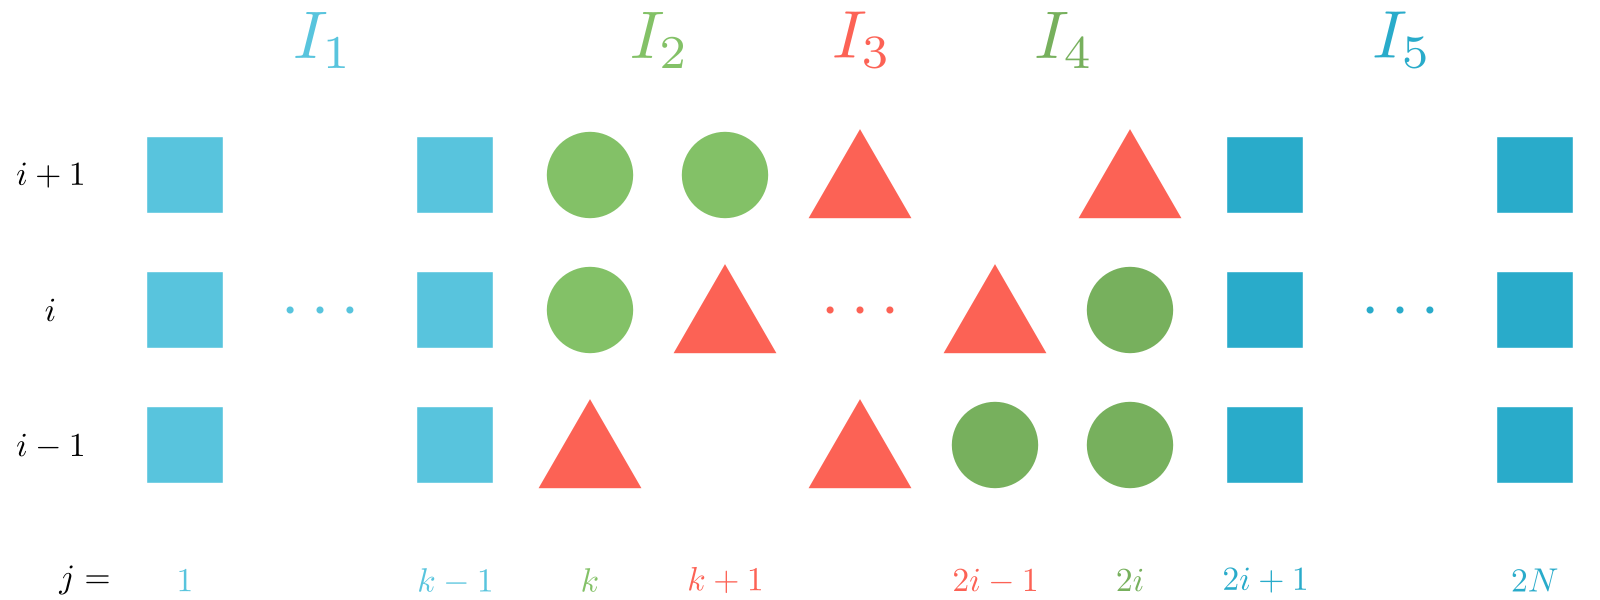
\includegraphics[width=0.8\textwidth]{Depart.png}
  \caption{The departure of \(R_i\) for \(i\ge 3\)}
\end{figure}
and discuss \(i=1,2\) separately, where
\begin{equation} \label{eq:departR1R2}
  R_1 = \sum_{i=1}^3 V_{1,j} + \sum_{i=4}^N V_{i,j}, \quad 
  R_2 = \sum_{i=1}^4 V_{1,j} + \sum_{i=5}^N V_{i,j}
\end{equation}

The difficulty for esitmating \(S_{ij}\) is that \(T_{i-1, j-1}, T_{i,j}\) and \(T_{i+1,j+1}\) have different integral region. 
We first make them normalized.

% To estimete \(S_{ij}\), we need some preparations.
\begin{lemma} \label{lmm:Tij-normalized}
  For \(y\in (x_{j-1}, x_{j})\), we can rewrite \(y=y_j^\theta\),
  from \eqref{def:Tij}, and \cref{lmm:Dyj},
  \begin{equation}
    \begin{aligned}
      T_{ij} & = \int_{x_{j-1}}^{x_{j}} (u(y) - \Pi_hu(y)) \frac{|y-x_i|^{1-\alpha}}{\Gamma(2-\alpha)} dy  \\
             & = \int_{0}^{1} (u(y_j^\theta) - \Pi_hu(y_j^\theta)) \frac{|y_j^\theta-x_i|^{1-\alpha}}{\Gamma(2-\alpha)} h_j d\theta  \\
      %        & = \int_{x_{j-1}}^{x_{j}}
      % -\frac{\theta (1-\theta)}{2} h_j^2 u''(y_j^\theta)\frac{|y_j^\theta-x_i|^{1-\alpha}}{\Gamma(2-\alpha)} \\
      %        & \quad + \frac{\theta (1-\theta)}{3!} h_j^3 \frac{|y_j^\theta-x_i|^{1-\alpha}}{\Gamma(2-\alpha)} ((1-\theta)^2 u'''(\eta_{j1}^\theta) - \theta^2  u'''(\eta_{j2}^\theta)) d y_j^\theta \\
             & = \int_{0}^{1}
      -\frac{\theta (1-\theta)}{2} h_j^3 u''(y_j^\theta)\frac{|y_j^\theta-x_i|^{1-\alpha}}{\Gamma(2-\alpha)}   \\
             & \quad + \frac{\theta (1-\theta)}{3!} h_j^4 \frac{|y_j^\theta-x_i|^{1-\alpha}}{\Gamma(2-\alpha)} ( \theta^2 u'''(\eta_{j1}^\theta) - (1-\theta)^2 u'''(\eta_{j2}^\theta)) d\theta
    \end{aligned}
  \end{equation}
  where \(\eta_{j1}^\theta \in (x_{j-1}, y_j^\theta), \eta_{j2}^\theta \in (y_j^\theta, x_j)\).
\end{lemma}

Since \(j\) changes with \(i\) at indices of elements in \(S_{ij}\) by \cref{def:Sij}, we create some functions satisfy the property.





\textcolor{purple}{
\begin{definition} [Mesh Transport Functions]
  For \(1\le i, j \le 2N-1\).
  \begin{equation} \label{def:yij}
    y_{i,j}(x) = \begin{cases}
      (x^{1/r} + Z_{j-i})^r               & i< N, j< N \\
      \dfrac{x^{1/r} - Z_i}{Z_1} h_N + x_N  & i< N, j=N \\
      2T - (Z_{2N-(j-i)} - x^{1/r})^r     & i< N, j>N \\
      \left(\dfrac{Z_1}{h_N}  (x-x_N) + Z_j \right)^r  & i=N, j< N \\
      x,                                  & i=N, j=N \\
      2T - \left(\dfrac{Z_1}{h_N}  (2T-x-x_N) + Z_{2N-j} \right)^r   & i=N , j > N \\
      (Z_{2N+j-i} - (2T - x)^{1/r})^r  & i > N, j< N \\
      \dfrac{Z_{2N-j} - (2T-x)^{1/r}}{Z_1} h_N + x_N  & i > N, j=N \\
      2T-((2T-x)^{1/r}-Z_{j-i})^r & i > N, j> N \\
    \end{cases}
  \end{equation}
  where  \( Z_{j} := T^{1/r}\frac{j}{N} \).
  And
  \begin{equation} \label{def:hij}
    h_{i,j}(x) = y_{i,j}(x) - y_{i,j-1}(x)
  \end{equation}
  \begin{equation} \label{def:yijt}
    y_{i,j}^\theta(x) = (1-\theta) y_{i,j-1}(x) + \theta y_{i,j-1}(x), \quad \theta \in (0, 1)
  \end{equation}
  \begin{equation} \label{def:Pj-itheta-jlN}
    {P_{i,j}^\theta}(x) = ({h_{i,j}}(x))^3  \frac{|{y_{i,j}^\theta}(x)-x|^{1-\alpha}}{\Gamma(2-\alpha)} u''({y_{i,j}^\theta}(x))
  \end{equation}
  \begin{equation} \label{def:Qj-itheta-jlN}
    {Q_{i,j;l}^\theta}(x) = ({h_{i,j}}(x))^l \frac{|{y_{i,j}^\theta}(x)-x|^{1-\alpha}}{\Gamma(2-\alpha)}
  \end{equation}
\end{definition}
}

Obviously,
\begin{gather}
  y_{i,j}(x_{i-1}) = x_{j-1}, \quad y_{i,j}(x_{i}) = x_{j}, \quad y_{i,j}(x_{i+1}) = x_{j+1} \\
  h_{i,j}(x_{i-1}) = h_{j-1}, \quad h_{i,j}(x_{i}) = h_j, \quad h_{i,j}(x_{i+1}) = h_{j+1} \\
  y_{i,j}^\theta(x_{i-1}) = y_{j-1}^\theta, \quad y_{i,j}^\theta(x_{i}) = y_{j}^\theta, \quad y_{i,j}^\theta(x_{i+1}) = y_{j+1}^\theta
\end{gather}


And now we can rewrite \(T_{ij}\)
\begin{lemma} 
  % For \(0\le i \le 2N\), \(1 \le j \le 2N\),
  \begin{equation} \label{lmm:Tij-express-as-int-of-function}
    \begin{aligned}
      T_{ij} & = \int_{0}^{1} -\frac{\theta (1-\theta)}{2} {P_{i,j}^\theta}(x_i) d\theta    \\
             & + \int_{0}^{1} \frac{\theta (1-\theta)}{3!}{Q_{i,j;l}^\theta}(x_i) \left[ \theta^2  u'''(\eta_{j,1}^\theta) - (1-\theta)^2 u'''(\eta_{j,2}^\theta) \right] d\theta
    \end{aligned}
  \end{equation}
  Immediately, we can see from \eqref{def:Sij} and \cref{lmm:Tij-normalized} that
  For \( 1 \le i \le 2N-1\), \(2\le j \le 2N-1\),
  \begin{equation} \label{lmm:Vij-int}
    \begin{aligned}
      S_{ij}
             & = \int_{0}^{1} -\frac{\theta (1-\theta)}{2} D_h^2 P_{i,j}^\theta(x_i)  d\theta    \\
             & \quad +  \int_{0}^1 \frac{\theta^3 (1-\theta)}{3!} \frac{2}{h_{i} + h_{i+1}}\left( \frac{{Q_{i,j;4}^\theta}(x_{i+1}) u'''(\eta_{j+1,1}^\theta) - {Q_{i,j;4}^\theta}(x_{i}) u'''(\eta_{j,1}^\theta)}{h_{i+1}}\right)  d\theta \\
             & \quad -  \int_{0}^1 \frac{\theta^3 (1-\theta)}{3!} \frac{2}{h_{i} + h_{i+1}}\left( \frac{{Q_{i,j;4}^\theta}(x_{i}) u'''(\eta_{j,1}^\theta) - {Q_{i,j;4}^\theta}(x_{i-1}) u'''(\eta_{j-1,1}^\theta)}{h_{i}}\right)  d\theta   \\
             & \quad -  \int_{0}^1 \frac{\theta (1-\theta)^3}{3!} \frac{2}{h_{i} + h_{i+1}}\left( \frac{{Q_{i,j;4}^\theta}(x_{i+1}) u'''(\eta_{j+1,2}^\theta) - {Q_{i,j;4}^\theta}(x_{i}) u'''(\eta_{j,2}^\theta)}{h_{i+1}}\right)  d\theta \\
             & \quad +  \int_{0}^1 \frac{\theta (1-\theta)^3}{3!} \frac{2}{h_{i} + h_{i+1}}\left( \frac{{Q_{i,j;4}^\theta}(x_{i}) u'''(\eta_{j,2}^\theta) - {Q_{i,j;4}^\theta}(x_{i-1}) u'''(\eta_{j-1,2}^\theta)}{h_{i}}\right)  d\theta
    \end{aligned}
  \end{equation}
\end{lemma}




We give some properties of mesh transport functions.

\begin{lemma} \label{lmm:gen-prop-of-MTFs}
  For \(2 \le i,j \le 2N-2\) and \(\xi \in (x_{i-1}, x_{i+1})\)
  \begin{equation}
    \xi \simeq x_i, \quad \delta(y_{i,j}(\xi))\simeq \delta(x_j), \quad h_{i,j}(\xi) \simeq h_j
  \end{equation}
  % For \(1\le i, j \le 2N-1\),
  \begin{equation}
    |y_{i,j}(\xi) - \xi| \simeq |x_j - x_i|, \quad |y_{i,j-1}(\xi) - \xi| \simeq |x_{j-1} - x_i|
  \end{equation}  then % for \(1\le i\le 2N-1, 2\le j \le 2N-1\),
  \begin{equation}
    |y_{i,j}^\theta(\xi) - \xi| = (1-\theta)|y_{i,j-1}(\xi) - \xi| + \theta |y_{i,j}(\xi) - \xi| \simeq |y_j^\theta - x_i|
  \end{equation}
  since \(y_{i,j-1}(\xi) - \xi\), \(y_{i,j}(\xi) - \xi\) have the same sign \((\ge 0\) or \(\le 0)\)
\end{lemma}

\begin{lemma} \label{lmm:derivatives-of-MTFs}
  \begin{equation}
    y_{i,j}'(x) = \begin{cases}
      y_{i,j}^{1-1/r}(x) x^{1/r-1}   & i< N, j< N \\
      \dfrac{h_N}{r Z_1} x^{1/r-1}  & i< N, j=N \\
      (2T-y_{i,j}(x))^{1-1/r} x^{1/r-1}   & i< N, j>N \\
      y_{i,j}^{1-1/r}(x) \dfrac{r Z_1}{h_N}  & i=N, j< N \\
      1   & i=N, j=N 
    \end{cases}
  \end{equation}
  \begin{equation}
    y_{i,j}''(x) = \frac{1-r}{r}
      \begin{cases}
        y_{i,j}^{1-2/r}(x) x^{1/r-2} Z_{j-i}   & i< N, j< N \\
        \dfrac{h_N}{r Z_1} x^{1/r-2}  & i< N, j=N \\
        (2T-y_{i,j}(x))^{1-2/r} x^{1/r-2} Z_{2N-j+i}   & i< N, j>N \\
        -y_{i,j}^{1-2/r}(x) \left(\dfrac{r Z_1}{h_N}\right)^2  & i=N, j< N \\
        0   & i=N, j=N 
      \end{cases}
  \end{equation}
\end{lemma}


% \textcolor{red}{
\begin{lemma} \label{lmm:esitmate-of-MTFs-1}
  For  \(2\le i \le N, 2\le j \le 2N-2\), \(\xi \in (x_{i-1}, x_{i+1}) \) 
  \begin{equation}
    |h_{i,j}'(\xi)| \le C (r-1) Z_1 x_i^{1/r-1}  \delta(x_j)^{1-2/r}
    \le C(r-1) h_j x_i^{1/r-1} \delta(x_j)^{-1/r}
  \end{equation}
  \begin{equation}
    \left|(y_{i,j}(\xi) - \xi)'\right| \le C x_i^{-1} |x_j - x_i|
  \end{equation}
\end{lemma}
% }
\begin{proof}
  From \eqref{def:hij} and \cref{lmm:derivatives-of-MTFs}, we can see that
  \begin{equation}
    \begin{aligned}
      h_{i,j}'(x) &= y_{i,j}'(x) - y_{i,j-1}'(x) \\ 
      &=\begin{cases}
        x^{1/r-1} ( y_{i,j}^{1-1/r}(x) - y_{i,j-1}^{1-1/r}(x) ) & i< N, j< N \\
        x^{1/r-1} ( \dfrac{h_N}{r Z_1} - y_{i,N-1}^{1-1/r}(x) )  & i< N, j=N \\
        x^{1/r-1} \left( (2T-y_{i,N+1}(x))^{1-1/r} - \dfrac{h_N}{r Z_1}  \right)   & i< N, j=N+1 \\
        x^{1/r-1} \left( (2T-y_{i,j}(x))^{1-1/r} - (2T-y_{i,j-1}(x))^{1-1/r} \right)   & i< N, j>N+1 \\
        \dfrac{rZ_1}{h_N} \left( y_{N,j}^{1-1/r}(x) - y_{N,j-1}^{1-1/r}(x) \right)  & i=N, j< N \\
        \dfrac{rZ_1}{h_N} \left( \dfrac{h_N}{rZ_1} - y_{N,N-1}^{1-1/r}(x) \right)   & i=N, j=N 
      \end{cases}
    \end{aligned}
  \end{equation}
  While for \(2\le i\le N\), if \(2\le j < N\), \(\xi \in (x_{i-1}, x_{i+1})\),
  \begin{equation} \label{eq:yij1-1/r-j-1}
    \begin{aligned}
      y_{i,j}^{1-1/r}(\xi) - y_{i,j-1}^{1-1/r}(\xi)
      &\le x_{j+1}^{1-1/r} - x_{j-2}^{1-1/r}  \\
      &= T^{1-1/r} N^{1-r} \left( (j+1)^{r-1} - (j-2)^{r-1} \right) \\
      & \le C T^{1-1/r} (r-1) N^{1-r} j^{r-2} = C  (r-1) Z_1 x_j^{1-2/r}
    \end{aligned}
  \end{equation}
  % and similar for \(N+1 < j \le 2N-1\).
  if \(j=N\), \(\xi \in (x_{i-1}, x_{i+1})\), we have \(y_{i,N-1}(\xi) \in (x_{N-2}, x_{N})\). And 
  \begin{equation} \label{eq:hN/rZ1}
    \dfrac{h_N}{r Z_1} = T^{1-1/r} \dfrac{1 - (1-h)^r}{rh} = \eta^{1-1/r} \simeq x_N^{1-1/r}, \quad \eta \in (x_{N-1}, x_{N})
  \end{equation}
  Then
  \begin{equation} \label{eq:hN/rZ1-yj=N-1}
    |\dfrac{h_N}{r Z_1} - y_{i,N-1}^{1-1/r}(\xi)| \le x_N^{1-1/r} - x_{N-2}^{1-1/r} \simeq (r-1) Z_1 x_N^{1-2/r}
  \end{equation}
  and similar for \(j\ge N+1\).
  Combine with \cref{lmm:hilexi}, \cref{lmm:gen-prop-of-MTFs}, \(\eta \simeq x_N\), we get the first result.

  For the second estimate, we have
  \begin{equation}
      (y_{i,j}(x) - x)' = y_{i,j}'(x) - 1
  \end{equation}
  Then, for \(2\le i < N\), if \(2\le j<N\), \(\xi \in (x_{i-1}, x_{i+1})\), by \cref{ineq:a-b-theta}
  \begin{equation}
    \xi^{1/r} |y_{i,j}^{1-1/r}(\xi) - \xi^{1-1/r}| \le |y_{i,j}(\xi) - \xi|
  \end{equation}
  \(j>N\) is symmetric to it, that is
  \begin{equation} \label{eq:2T-yij1-1/r}
    \begin{aligned}
      &\xi^{1/r} |(2T-y_{i,j}(\xi))^{1-1/r} - \xi^{1-1/r}|
              \le |2T - y_{i,j}(\xi) - \xi|  \\
      & \quad \le |2T - x_j - x_i| + |y_{i,j}(\xi) - x_j| + |\xi - x_i|
              \le |2T - x_j - x_i| + 2 h_N   \\
      & \quad \le |x_j - T| + |T-x_i| + 2h_N \le 2 |x_j - x_i|
    \end{aligned}
  \end{equation}

  But if \(j=N\), with \cref{eq:hN/rZ1} and \cref{ineq:a-b-theta},
  \begin{equation} \label{eq:hN/rZ1-xi<N}
    \begin{aligned}
      \eta^{1/r} |\dfrac{h_N}{r Z_1} - \xi^{1-1/r}| &\le |\eta - \xi|, \quad \eta \in (x_{N-1}, x_{N})  \\
      & \le |x_N - x_i| + |h_N| + |h_{i+1}| \le 3 |x_N - x_i|
    \end{aligned}
  \end{equation}

  For \(i=N\), if \(j<N\), similarly with \cref{eq:hN/rZ1-xi<N},
  \begin{equation}
    \eta^{1/r} |y_{N, j}^{1-1/r}(\xi) - \dfrac{h_N}{r Z_1}| \le C |x_j - x_N|
  \end{equation}
  And if \(j=N\), it is obviously \(\equiv 0\).

  Similarly, by \cref{lmm:derivatives-of-MTFs} and \cref{lmm:gen-prop-of-MTFs}, we get the second result.
\end{proof}

\begin{lemma} \label{lmm:esitmate-of-MTFs-2}
  For \(2\le i \le N, 2\le j \le 2N-2\), \(\xi \in (x_{i-1}, x_{i+1})\)
  \begin{equation}
    |y_{i,j}''(\xi)| \le C(r-1)
    \begin{cases}
      x_j^{-1/r} x_i^{1/r-2} |x_j - x_i|  & i < N, j < N  \\
      x_N^{1-1/r} x_i^{1/r-2}             & i < N, j = N  \\
      \delta(x_j)^{1-2/r} x_i^{1/r-2} x_N^{1/r}     & i < N, j > N  \\
      \delta(x_j)^{1-2/r} x_N^{2/r-2}             & i = N, j \neq N  \\
      0   & i = N, j = N
    \end{cases}
  \end{equation}
  And \(2\le i \le N, 3\le j \le 2N-2\), \(\xi \in (x_{i-1}, x_{i+1}) \) 
  \begin{equation}
    |h_{i,j}''(\xi)| \le C (r-1)
    \begin{cases}
      Z_1 x_i^{1/r-2} x_j^{-2/r} (|x_j - x_i| + x_j)   & i < N, j < N  \\
      x_i^{1/r-2} x_N^{1-1/r}                        & i < N, j=N, N+1 \\
      Z_1 x_i^{1/r-2} \delta(x_j)^{1-3/r}  x_N^{1/r}    & i < N, j>N+1 \\
      Z_1 x_N^{2/r-2} \delta(x_j)^{1-3/r}               & i = N, j < N \text{  or  } j > N+1  \\
      x_N^{-1}                                       & i = N, j = N
    \end{cases}
  \end{equation}
\end{lemma}
\begin{proof}
  Since by \cref{ineq:a-b-theta}, for \(2 \le i, j < N\)
  \begin{equation} \label{eq:Zj-i}
    x_j^{1-1/r} |Z_{j-i}| = x_j^{1-1/r} |x_j^{1/r} - x_i^{1/r}| \le |x_j - x_i|
  \end{equation}
  and by \eqref{eq:hN/rZ1}, \(\dfrac{h_N}{r Z_1} \simeq x_N^{1-1/r}\). And
  \begin{equation}
    Z_{2N-j+i} \le Z_{2N} =  2 T^{1/r}
  \end{equation}
  Then by \cref{lmm:derivatives-of-MTFs} and \cref{lmm:gen-prop-of-MTFs}, we get the first result.

  For the second part, by \cref{lmm:derivatives-of-MTFs}
  \begin{equation}
    \begin{aligned}
      h_{i,j}''(x) &= y_{i,j}''(x) - y_{i,j-1}''(x)
    \end{aligned}
  \end{equation}
  while for \(2\le i<N\), if \(3\le j<N\), \(\xi\in (x_{i-1}, x_{i+1})\),
  \begin{equation} \label{eq:yij1-2/rZj-i-depart}
    \begin{aligned}
      y_{i,j}^{1-2/r}(\xi) Z_{j-i} - y_{i,j-1}^{1-2/r}(\xi) Z_{j-i-1}
      = \left( y_{i,j}^{1-2/r}(\xi) - y_{i,j-1}^{1-2/r}(\xi) \right) Z_{j-i} + y_{i, j-1}^{1-2/r}(\xi) Z_1
    \end{aligned}
  \end{equation}
  where \(y_{i,j}^{1-2/r}(\xi) - y_{i,j-1}^{1-2/r}(\xi) \simeq (r-2) Z_1 x_j^{1-3/r} \) similar with \cref{eq:yij1-1/r-j-1}. Combine with \cref{eq:Zj-i}, we get
  \begin{equation} \label{eq:yij1-2/rZj-i-}
    |y_{i,j}^{1-2/r}(\xi) Z_{j-i} - y_{i,j-1}^{1-2/r}(\xi) Z_{j-i-1}| \le C Z_1 \left( |r-2| x_j^{-2/r}|x_j - x_i| + x_j^{1-2/r}  \right)
  \end{equation}
  if \(j=N\), 
  \begin{equation}
    \begin{aligned}
      |h_{i,N}''(x)| &\le |y_{i,N}''(x)| + |y_{i,N-1}''(x)| \le C (r-1) x_i^{1/r-2} x_N^{1-1/r}
    \end{aligned}
  \end{equation}
  similarly if \(j= N+1\).

  However, if \(j > N+1\), similar with \cref{eq:yij1-2/rZj-i-depart}, we get
  \begin{equation}
    \begin{aligned}
      &(2T-y_{i,j}(\xi))^{1-2/r} Z_{2N-(j-i)} - (2T-y_{i,j-1}(\xi))^{1-2/r} Z_{2N-(j-i-1)} \\
      & = \left( (2T-y_{i,j}(\xi))^{1-2/r} - (2T-y_{i,j-1}(\xi))^{1-2/r} \right) Z_{2N-(j-i)} - (2T-y_{i, j-1}(\xi))^{1-2/r} Z_1
    \end{aligned}
  \end{equation}
  thus, 
  \begin{equation}
    \begin{aligned}
      &\left|(2T-y_{i,j}(\xi))^{1-2/r} Z_{2N-(j-i)} - (2T-y_{i,j-1}(\xi))^{1-2/r} Z_{2N-(j-i-1)} \right| \\
      &\le C Z_1 \left( |r-2| (2T-x_j)^{1-3/r} x_N^{1/r} + (2T-x_j)^{1-2/r}  \right) \le C Z_1 (2T-x_j)^{1-3/r} x_N^{1/r}
    \end{aligned}
  \end{equation}
  For \(i=N\), it's obvious.
  Combine with \cref{lmm:derivatives-of-MTFs} and \cref{lmm:gen-prop-of-MTFs}, we get the second result.
\end{proof}














\subsection{Proof of Theorems}

Then we esrimate each part of \eqref{eq:depart-Ri}. And We take
\(m = 2i\) for \(3 \le i < N/2\), and \(m = N-\lceil N/2 \rceil +1\) for \(N/2 \le i\le N\).

For \(I_5\)
\textcolor{blue}{
  \begin{lemma} \label{lmm:Ri-I5-1}
    There exists a constant \(C=C(T, \alpha, r, \|u\|_{\beta+\alpha}^{(-\alpha/2)})\) such that
    \paragraph{Case 1}
    For  \(1 \le i < N/2\),
    \begin{equation}
      \begin{aligned}
        \sum_{j=\max\{2i+1, 4\}}^{N} \left| V_{ij} \right| 
        \le C h^2 x_i^{-\alpha/2-2/r}
      \end{aligned}
    \end{equation}
    \paragraph{Case 2}
    For \(1 \le i < N/2\),
    \begin{equation}
      \begin{aligned}
        \sum_{j=N+1}^{2N} |V_{ij}|
        \le \begin{cases}
              C h^2,             & \alpha/2-2/r+1 > 0 \\
              C h^2 \ln(N) ,     & \alpha/2-2/r+1 = 0 \\
              C h^{r\alpha/2+r}, & \alpha/2-2/r+1 < 0
            \end{cases}
      \end{aligned}
    \end{equation}
    \paragraph{Case 3}
    For \(N/2 \le i \le N\),
    \begin{equation}
      \begin{aligned}
        \sum_{j=N-\lceil\frac{N}{2}\rceil+2}^{2N} |V_{ij}|
        \le \begin{cases}
              C h^2,             & \alpha/2-2/r+1 > 0 \\
              C h^2 \ln(N) ,     & \alpha/2-2/r+1 = 0 \\
              C h^{r\alpha/2+r}, & \alpha/2-2/r+1 < 0
            \end{cases}
      \end{aligned}
    \end{equation}
  \end{lemma}
}
\begin{proof}
  For \(i,j\) in each case, by \cref{def:Vij}, \cref{lmm:Dyjleh2ya/2m2/r} and \cref{lmm:Dh2Kyxi}, we have
  \begin{equation}
    \begin{aligned}
      | V_{ij}| 
      % & = \left| \int_{x_{j-1}}^{x_{j}}(u(y) - \Pi_hu(y)) D_h^2 K_y (x_i) dy \right| \\
              & \le C h^2 \int_{x_{j-1}}^{x_{j}} \delta(y)^{\alpha/2-2/r} |y-x_i|^{-1-\alpha} dy                       \\
            %  & = C h^2 \int_{x_{j-1}}^{x_{j}} y^{-\alpha/2-2/r-1} dy
    \end{aligned}
  \end{equation}
  For Case 1, with \(x_{i} \simeq x_{2i} \),
  \begin{equation}
    \begin{aligned}
      \sum_{j=\max\{2i+1, 4\}}^{N} |V_{ij}|
        & \le C h^2 \int_{x_{2i}}^{x_{N}} y^{-\alpha/2-2/r-1} dy                     \\
        & = \frac{C}{\alpha/2+2/r} h^2 ( x_{2i}^{-\alpha/2-2/r} - T^{-\alpha/2-2/r}) \\
        & \le C h^2 x_i^{-\alpha/2-2/r}
    \end{aligned}
  \end{equation}
  For Case 2 , by \cref{def:Vij}, \cref{lmm:Dyjleh2ya/2m2/r}, \cref{lmm:Dh2Kyxi} and \(y-x_i\simeq T\)
  \begin{equation*}
    \begin{aligned}
      |V_{ij}| 
      % & = \left| \int_{x_{j-1}}^{x_{j}}(u(y) - \Pi_hu(y)) D_h^2 K_y (x_i) dy \right| \\
            %  & \le C \int_{x_{j-1}}^{x_{j}} h^2 (2T-y)^{\alpha/2-2/r} |y-x_i|^{-1-\alpha} dy                                          \\
             & \le C h^2  T^{-1-\alpha} \int_{x_{j-1}}^{x_{j}} (2T-y)^{\alpha/2-2/r} dy
    \end{aligned}
  \end{equation*}
  \begin{equation}
    \begin{aligned}
      \sum_{j=N+1}^{2N-1} |V_{ij}|
       & \le C T^{-1-\alpha} h^2 \int_{x_{N}}^{x_{2N-1}} (2T-y)^{\alpha/2-2/r}  dy                       \\
       & \le CT^{-1-\alpha} h^2 \begin{cases}
                                  \frac{1}{\alpha/2-2/r+1} T^{\alpha/2-2/r+1},        & \alpha/2-2/r+1 > 0 \\
                                  \ln(T)-\ln(h_{2N}),                                 & \alpha/2-2/r+1 = 0 \\
                                  \frac{1}{|\alpha/2-2/r+1|} h_{2N}^{\alpha/2-2/r+1}, & \alpha/2-2/r+1 < 0
                                \end{cases} \\
       & = \begin{cases}
             \frac{C}{\alpha/2-2/r+1}T^{-\alpha/2-2/r} \; h^2,                & \alpha/2-2/r+1 > 0 \\
             CrT^{-1-\alpha} h^2 \ln(N),                                      & \alpha/2-2/r+1 = 0 \\
             \frac{C}{|\alpha/2-2/r+1|} T^{-\alpha/2-2/r} \; h^{r\alpha/2+r}, & \alpha/2-2/r+1 < 0
           \end{cases}
    \end{aligned}
  \end{equation}
  And by \cref{lmm:Dyj1}
  \begin{equation*}
    |V_{i,2N}| \le C T^{-1-\alpha} h_{2N}^{\alpha/2+1} = C T^{-\alpha/2} h^{r\alpha/2+r}
  \end{equation*}
  Summarizes, we get the result.
  Similar for Case 3.
\end{proof}



For \(i=1, 2\).

\begin{lemma} \label{lmm:R1R2}
  From \eqref{eq:departR1R2},  by \cref{lmm:sumSij13}, \cref{lmm:Ri-I5-1} Case 1 2,  we get for \(i=1, 2\)
  \begin{equation}
    \begin{aligned}
      |R_i| \le C h^2 x_i^{-\alpha/2-2/r} +
      \begin{cases}
        C h^2,             & \alpha/2-2/r+1 > 0 \\
        C h^2 \ln(N) ,     & \alpha/2-2/r+1 = 0 \\
        C h^{r\alpha/2+r}, & \alpha/2-2/r+1 < 0
      \end{cases}
    \end{aligned}
  \end{equation}
\end{lemma}



\textcolor{blue}{
  \begin{lemma} \label{lmm:Ri-I1}
    There exists a constant \(C=C(T, \alpha, r, \|u\|_{\beta+\alpha}^{(-\alpha/2)})\) such that for \(3\le i \le N, k=\lceil\frac{i}{2}\rceil\)
    \begin{equation}
      |I_1| = |\sum_{j=1}^{k-1} V_{ij}| \le \begin{cases}
        C h^2 x_i^{-\alpha/2-2/r} ,        & \alpha/2-2/r+1 > 0 \\
        C h^2 x_i^{-1-\alpha} \ln(i),      & \alpha/2-2/r+1 = 0 \\
        C h^{r\alpha/2+r} x_i^{-1-\alpha}, & \alpha/2-2/r+1 < 0
      \end{cases}
    \end{equation}
  \end{lemma}
}
\begin{proof}
  by \cref{def:Vij}, \cref{lmm:Dyj1} , \cref{lmm:Dh2Kyxi}
  \begin{equation}
    |V_{i1}| \le C \int_{0}^{x_1} x_1^{\alpha/2} |x_i-y|^{-1-\alpha}dy \simeq x_1^{\alpha/2+1} x_i^{-1-\alpha} = T^{\alpha/2+1} h^{r\alpha/2+r} x_i^{-1-\alpha}
  \end{equation}
  For  \(2 \le j \le k-1\), by \cref{lmm:Dyjleh2ya/2m2/r} and \cref{lmm:Dh2Kyxi} with \(x_i - y \simeq x_i\), we have
  \begin{equation}
    \begin{aligned}
      |V_{ij}| 
      % & = \left|  \int_{x_{j-1}}^{x_{j}}(u(y) - \Pi_hu(y)) D_h^2 K_y(x_i) dy  \right| \\
             & \le C h^2 \int_{x_{j-1}}^{x_{j}} y^{\alpha/2-2/r} x_i^{-1-\alpha} dy
    \end{aligned}
  \end{equation}
  Therefore,
  \begin{equation}
    \begin{aligned}
      \sum_{j=2}^{k-1} |V_{ij}|
        \le C h^{r\alpha/2+r} x_i^{-1-\alpha} + C h^2 x_i^{-1-\alpha} \int_{x_1}^{x_{\lceil\frac{i}{2}\rceil-1}} y^{\alpha/2-2/r} dy
    \end{aligned}
  \end{equation}
  But \(x_{\lceil\frac{i}{2}\rceil-1} \le 2^{-r} x_i\), so we have
  \begin{equation}
    \begin{aligned}
      \int_{x_1}^{x_{\lceil\frac{i}{2}\rceil-1}} y^{\alpha/2-2/r} dy
       & \le \begin{cases}
               \frac{1}{\alpha/2-2/r+1} (2^{-r} x_i)^{\alpha/2-2/r+1} , & \alpha/2-2/r+1 > 0 \\
               \ln(2^{-r} x_i) - \ln(x_1),                              & \alpha/2-2/r+1 = 0 \\
               \frac{1}{|\alpha/2-2/r+1|} x_1^{\alpha/2-2/r+1},         & \alpha/2-2/r+1 < 0
             \end{cases}
    \end{aligned}
  \end{equation}
  Combine the results above, we get the lemma.
\end{proof}


\textcolor{blue}{
  \begin{lemma} \label{lmm:d2Pj-itle}
    There exists a constant \(C=C(T, \alpha, r, \|u\|_{\beta+\alpha}^{(-\alpha/2)})\) such that
    \paragraph{Case 1}
    For \(3\le i < N, \lceil\frac{i}{2}\rceil+1 \le j \le \min\{2i-1, N-1\}\),
    \begin{equation}
      |D_h^2 {P_{i,j}^\theta}(x_{i})| \le C h_j^3 \frac{|y_j^\theta - x_i|^{1-\alpha}}{\Gamma(2-\alpha)} x_i^{\alpha/2-4}
    \end{equation}
    \paragraph{Case 2}
    For \(N/2\le i \le N\), \(j=N, N+1\)
    \begin{equation}
      \begin{aligned}
        |D_h^2 P_{i,j}^\theta(\xi)| 
        \le C h_j^3 |y_j^\theta - x_i|^{1-\alpha}  + C(r-1) h_j^2 \Big(|y_j^\theta - x_i|^{1-\alpha} + h_j|y_j^\theta - x_i|^{-\alpha}
        \Big)
      \end{aligned}
    \end{equation}
    \paragraph{Case 3}
    For \(N/2 \le i \le N\), \(N+2 \le j \le 2N-\lceil\frac{N}{2}\rceil\),
    \begin{equation}
      \begin{aligned}
        |D_h^2 P_{i,j}^\theta(\xi)| 
        \le C h_j^3 \Big(|y_j^\theta - x_i|^{1-\alpha}  + (r-1) |y_j^\theta - x_i|^{-\alpha}
        \Big)
      \end{aligned}
    \end{equation}
    % \paragraph{Case 4}
    % For \(i=N\), \(N/2 \le j < N\)
    % where \(y_j^\theta = \theta x_{j-1} + (1-\theta) x_{j}\)
  \end{lemma}
}
\begin{proof}
  Since \(\text{sign}(y_{i,j}^\theta(\xi) - \xi)\) is independent of \(\xi\), we can derivate it. 
  Then by \cref{lmm:Dh2simd2}
  \begin{equation}
    D_h^2 {P_{i,j}^\theta}(x_i) = {P_{i,j}^\theta}''(\xi), \quad \xi\in (x_{i-1}, x_{i+1})
  \end{equation}
  From \eqref{def:Pj-itheta-jlN}, using Leibniz formula and chain rules, and 
  \cref{lmm:gen-prop-of-MTFs}, 
  \cref{lmm:derivatives-of-MTFs},
  \cref{lmm:esitmate-of-MTFs-1}, 
  \cref{lmm:esitmate-of-MTFs-2}, 
  \cref{cor:regularity-u},
  \cref{lmm:hilexi}

  For every case, we have \(x_i \simeq \delta(x_j)\), so we have
  \begin{equation}
    h_{i,j}(\xi) \le C h_j, \quad |h_{i,j}'(\xi)| \le C(r-1) h_j x_i^{-1}
  \end{equation}
  \begin{equation}
    |y_{i,j}^\theta(\xi) - \xi| \le C |y_j^\theta - x_i|, \quad 
    \left|(y_{i.j}^\theta(\xi) - x_i)'\right| \le C |y_j^\theta - x_i| x_i^{-1}
  \end{equation}
  \begin{equation}
    |u''(y_{i,j}^\theta(\xi))| \le C x_i^{\alpha/2-2}, \quad
    \left|\left(u''(y_{i,j}^\theta(\xi))\right)'\right| \le C x_i^{\alpha/2-3}, \quad 
    \left|\left(u''(y_{i,j}^\theta(\xi))\right)''\right| \le C x_i^{\alpha/2-4}
  \end{equation}
  
  By \cref{lmm:esitmate-of-MTFs-2}, we have

  For Case 1, 
  \begin{equation}
    |h_{i,j}''(\xi)| \le C(r-1) h_j x_i^{-2}, \quad 
    \left|(y_{i,j}^\theta(\xi) - x_i)''\right| \le C(r-1) |y_j^\theta - x_i| x_i^{-2}
  \end{equation}
  
  For Case 2, since \(x_i \simeq x_j \simeq T\)
  \begin{equation}
    |h_{i,j}''(\xi)| \le C(r-1), \quad 
    \left|(y_{i,j}^\theta(\xi) - x_i)''\right| \le C(r-1)
  \end{equation}
  
  For Case 3, since \(x_i \simeq \delta(x_j) \simeq T\), we have
  \begin{equation}
    |h_{i,j}''(\xi)| \le C(r-1) h_j, \quad 
    \left|(y_{i,j}^\theta(\xi) - x_i)''\right| \le C(r-1)
  \end{equation}
  Combine them, we get the result.

\end{proof}

  
  \textcolor{blue}{
    \begin{lemma} \label{lmm:dQj-itle}
      There exists a constant \(C=C(T, \alpha, r, \|u\|_{\beta+\alpha}^{(-\alpha/2)})\) such that for \(2 \le i \le N\), \(2 \le j \le 2N-2\),
      \begin{equation}
        \begin{aligned}
          \left| \frac{{Q_{i,j;l}^\theta}(x_{i+1}) u^{(l-1)}(\eta_{j+1}^\theta) - {Q_{i,j;l}^\theta}(x_{i}) u^{(l-1)}(\eta_{j}^\theta)}{h_{i+1}}\right|
          \le C h_j^l \frac{|y_j^\theta - x_i|^{1-\alpha}}{\Gamma(2-\alpha)} x_i^{-1} \delta(x_j)^{\alpha/2-l+1-1/r} (x_i^{1/r} + \delta(x_j)^{1/r})
        \end{aligned}
      \end{equation}
      And
      \begin{equation}
        \begin{aligned}
          \left| \frac{{Q_{i,j;l}^\theta}(x_{i}) u^{(l-1)}(\eta_{j}^\theta) - {Q_{i,j;l}^\theta}(x_{i-1}) u^{(l-1)}(\eta_{j-1}^\theta)}{h_{i}} \right|
          \le C h_j^l \frac{|y_j^\theta - x_i|^{1-\alpha}}{\Gamma(2-\alpha)} x_i^{-1} \delta(x_j)^{\alpha/2-l+1-1/r} (x_i^{1/r} + \delta(x_j)^{1/r})
        \end{aligned}
      \end{equation}
      where \(\eta_{j}^\theta \in (x_{j-1}, x_{j})\).
    \end{lemma}
    }
    \begin{proof} \label{prf:dQj-itle}
      % For \(\lceil\frac{i}{2}\rceil+1 \le j \le \min\{2i-1, N-1\}\)
      \begin{equation}
        \begin{aligned}
           & \frac{{Q_{i,j;l}^\theta}(x_{i+1}) u'''(\eta_{j+1}^\theta) - {Q_{i,j;l}^\theta}(x_{i}) u'''(\eta_{j}^\theta)}{h_{i+1}}  \\
           & \quad = \frac{Q_{i,j;l}^\theta(x_{i+1}) - Q_{i,j;l}^\theta(x_{i})}{h_{i+1}} u'''(\eta_{j+1}^\theta)
          + Q_{i,j;l}^\theta(x_i) \frac{u'''(\eta_{j+1}^\theta)-u'''(\eta_{j}^\theta)}{h_{i+1}}                                   \\
          %  & \quad \le {Q_{i,j;l}^\theta}'(\xi) C x_j^{\alpha/2-3} + Q_{i,j;l}^\theta(x_i) C u''''(\eta)\frac{h_i+h_{i+1}}{h_{i+1}}
        \end{aligned}
      \end{equation}
      Using mean value theorem
      \begin{equation}
        D_h Q_{i,j;l}^\theta (x_i) :=   \frac{Q_{i,j;l}^\theta(x_{i+1}) - Q_{i,j;l}^\theta(x_{i})}{h_{i+1}} = {Q_{i,j;l}^\theta}'(\xi), \quad \xi \in (x_{i}, x_{i+1})
      \end{equation}
      From \eqref{def:Qj-itheta-jlN} and Leibniz rule, by \cref{lmm:gen-prop-of-MTFs}, \cref{lmm:esitmate-of-MTFs-1} and \cref{lmm:hilexi}, we have
      \begin{equation}
        \begin{aligned}
          |{Q_{i,j;l}^\theta}'(\xi)| \le C h_j^l \frac{|y_{j}^\theta - x_{i}|^{1-\alpha}}{\Gamma(2-\alpha)} (x_i^{-1} + x_i^{1/r-1} \delta(x_j)^{-1/r})
        \end{aligned}
      \end{equation}
      % And
      \begin{equation}
        Q_{i,j;l}^\theta(x_i) = h_{j}^l \frac{|y_j^\theta-x_i|^{1-\alpha}}{\Gamma(2-\alpha)}
      \end{equation}
      With \cref{lmm:hilexi} and \cref{cor:regularity-u}
      \begin{equation*}
        |u^{(l-1)}(\eta_{j+1}^\theta)| \le C (\eta_{j+1}^\theta)^{\alpha/2-l+1} 
        \simeq \delta(x_j)^{\alpha/2-l+1}
      \end{equation*}
      and by \cref{lmm:hilexi}
      \begin{equation*}
        \begin{aligned}
          \frac{|u^{(l-1)}(\eta_{j+1}^\theta)-u^{(l-1)}(\eta_{j}^\theta)|}{h_{i+1}}
          &= |u^{(l)}(\eta)| \frac{\eta_{j+1}^\theta - \eta_{j}^\theta}{h_{i+1}}  , \quad \eta \in (x_{j-1}, x_{j+1})\\
          & \le C \delta(\eta)^{\alpha/2-l} \frac{x_{j+1}-x_{j-1}}{h_{i+1}}
          = C \delta(\eta)^{\alpha/2-l} \frac{h_{j+1}+h_{j}}{h_{i+1}} \\
          & \simeq x_i^{1/r-1} \delta(x_j)^{\alpha/2-l+1-1/r} 
        \end{aligned}
      \end{equation*}
      Combine the results above, we get the first term.
      While, the later is similar.
    \end{proof}
    
    
    
    \textcolor{blue}{
  \begin{lemma} \label{lmm:estimate-Sij}
    There exists a constant \(C=C(T, \alpha, r, \|u\|_{\beta+\alpha}^{(-\alpha/2)})\)  such that 
    \paragraph{Case 1}
    For \(3\le i \le N-1, \lceil\frac{i}{2}\rceil+1 \le j \le \min\{2i-1, N-1\}\),
    \begin{equation} \label{eq:estimate-Sij-int}
      \begin{aligned}
        |S_{ij}| & \le C h_j^2 x_i^{\alpha/2-4} \int_{0}^{1}  \frac{|y_j^\theta - x_i|^{1-\alpha}}{\Gamma(2-\alpha)}  h_j d\theta \\
        & =  C h^2 x_i^{\alpha/2-2-2/r} \int_{x_{j-1}}^{x_{j}}  \frac{|y - x_i|^{1-\alpha}}{\Gamma(2-\alpha)}  dy
      \end{aligned}
    \end{equation}
    Thus,
    \begin{equation}
       \sum_{j=k+1}^{\min\{2i-1, N-1\}} \left|S_{ij} \right| \le C h^2 x_i^{-\alpha/2-2/r}
    \end{equation}
    \paragraph{Case 2}
    For \(N/2 \le i \le N\), \(j=N, N+1\),
    since \(\theta(1-\theta) h_j \le |y_j^\theta - x_i|\), we have
    \begin{equation}
      |S_{ij}| \le C (h^3 + (r-1)h^2) (T-x_i+h_N)^{1-\alpha}
    \end{equation}
    \paragraph{Case 3}
    For \(N/2 \le i \le N\), \(N+2 \le j \le 2N-\lceil\frac{N}{2}\rceil\),
    \begin{equation}
      |S_{ij}| \le C h^2 \int_{x_{j-1}}^{x_{j}} |y - x_i|^{1-\alpha} + (r-1)|y - x_i|^{-\alpha} dy
    \end{equation}
    Thus,
    \begin{equation}
      \sum_{j=N+2}^{2N-\lceil\frac{N}{2}\rceil} \left|S_{ij} \right| 
      \le C h^2 + C (r-1) h^2 (T-x_i + h_N)^{1-\alpha}
    \end{equation}
    Expecially, for \(i=N\), the estimate of \(\lceil\frac{N}{2}\rceil+1 \le j \le N-1\) is symmetric with \(N+2 \le j \le 2N-\lceil\frac{N}{2}\rceil\).
  \end{lemma}
  }
\begin{proof}
  Since \cref{lmm:Vij-int}, by \(x_i \simeq x_j\), \cref{lmm:hilexi}, \cref{lmm:d2Pj-itle}, \cref{lmm:dQj-itle}

  For Case 1,
  we get the first result immediately.
  While \(x_k \simeq x_i \simeq x_{\min\{2i-1, N-1\}}\), we have
  \begin{equation}
    \begin{aligned}
      \sum_{k+1}^{\min\{2i-1, N-1\}} |S_{ij}|
      &\le C h^2 x_i^{\alpha/2-2-2/r} \int_{x_{k}}^{x_{\min\{2i-1, N-1\}}} \frac{|y - x_i|^{1-\alpha}}{\Gamma(2-\alpha)}  dy    \\
        % & = C h^2 \left( \frac{|x_{k} - x_i|^{2-\alpha}}{\Gamma(3-\alpha)} + \frac{|x_{\min\{2i-1, N-1\}} - x_i|^{2-\alpha}}{\Gamma(3-\alpha)}\right) x_i^{\alpha/2-2-2/r} \\
        & \le C h^2  x_i^{\alpha/2-2-2/r}x_{i}^{2-\alpha} = C h^2 x_i^{-\alpha/2-2/r}
    \end{aligned}
  \end{equation}

  For Case 2,
  \begin{equation}
    \begin{aligned}
      |S_{ij}| &\le C (h_j^3 + (r-1)h_j^2) \int_{0}^1 |y_j^\theta - x_i|^{1-\alpha} d\theta \\
      &= C (h_j^2 + (r-1)h_j) \int_{x_{j-1}}^{x_{j}} |y - x_i|^{1-\alpha} dy \\
    \end{aligned}
  \end{equation}
  however, 
  \begin{equation}
    \begin{aligned}
      \int_{x_{j-1}}^{x_{j}} |y - x_i|^{1-\alpha} dy 
      &= \frac{1}{2-\alpha} \left((x_j-x_i)^{2-\alpha} - (x_{j-1}-x_i)^{2-\alpha}\right) \\
      &\simeq h_N (|x_j - x_i + h_N)^{1-\alpha}
    \end{aligned}
  \end{equation}

  For Case 3,
  \begin{equation}
    \begin{aligned}
      |S_{ij}| &\le C h_j^2 \int_{0}^1 \left(|y_j^\theta - x_i|^{1-\alpha}+ (r-1)|y_j^\theta - x_i|^{-\alpha}\right) h_j d\theta  \\
      &\le C h^2 \int_{x_{j-1}}^{x_{j}} |y - x_i|^{1-\alpha} + (r-1)|y - x_i|^{-\alpha} dy \\
    \end{aligned}
  \end{equation}
  Thus,
  \begin{equation}
    \begin{aligned}
      \sum_{j=N+2}^{2N-\lceil\frac{N}{2}\rceil} |S_{ij}| 
      &= C h^2 \int_{x_{N+1}}^{x_{2N-\lceil\frac{N}{2}\rceil}} |y - x_i|^{1-\alpha} + (r-1)|y - x_i|^{-\alpha} dy \\
      & \le C h^2 ( T^{2-\alpha} + (r-1) (T-x_i + h_N)^{1-\alpha} )  
    \end{aligned}
  \end{equation}
\end{proof}

Now we study \(I_2, I_4\).

  \begin{lemma} \label{lmm:Ri-I2-I4-ilN/2}
    There exists a constant \(C=C(T, \alpha, r, \|u\|_{\beta+\alpha}^{(-\alpha/2)})\) such that
    \paragraph{Case 1}
    For \(3\le i \le N, k=\lceil\frac{i}{2}\rceil\),
    \begin{equation}
      I_2 = \frac{2}{h_i + h_{i+1}}
      \left( \frac{1}{h_{i+1}} (T_{i+1, k} +  T_{i+1, k+1})
      - (\frac{1}{h_{i}}+\frac{1}{h_{i+1}}) T_{i,k} \right) \le C h^2 x_i^{-\alpha/2-2/r}
    \end{equation}
    \paragraph{Case 2}
    For \(3\le i < N/2\),
    \begin{equation}
      I_4 = \frac{2}{h_i + h_{i+1}}
      \left( \frac{1}{h_{i}} (T_{i-1, 2i} +  T_{i-1, 2i-1})
      - (\frac{1}{h_{i}}+\frac{1}{h_{i+1}}) T_{i,2i} \right) \le C h^2 x_i^{-\alpha/2-2/r}
    \end{equation}
    \paragraph{Case 3}
    For \(N/2 \le i \le N\), \(m=N-\lceil\frac{N}{2}\rceil+1\),
    \begin{equation}
      I_4 = \frac{2}{h_i + h_{i+1}}
      \left( \frac{1}{h_{i}} (T_{i-1, m} +  T_{i-1, m-1})
      - (\frac{1}{h_{i}}+\frac{1}{h_{i+1}}) T_{i,m} \right) \le C h^2
    \end{equation}
  \end{lemma}
  \begin{proof}
    In fact,
    \begin{equation}
      \begin{aligned}
         & \frac{1}{h_{i+1}} (T_{i+1, k} +  T_{i+1, k+1})
        - (\frac{1}{h_{i}}+\frac{1}{h_{i+1}}) T_{i,k}                                                                                                  \\
         & = \frac{1}{h_{i+1}} (T_{i+1, k} -  T_{i, k}) + \frac{1}{h_{i+1}} (T_{i+1, k+1} -  T_{i, k}) + (\frac{1}{h_{i+1}} - \frac{1}{h_{i}}) T_{i,k}
      \end{aligned}
    \end{equation}
    While, by \cref{lmm:Dyjleh2ya/2m2/r}, \cref{lmm:Dh2Kyxi}, \cref{lmm:hilexi} and \(x_k \simeq x_i\), we have
    \begin{equation}
      \begin{aligned}
        \frac{1}{h_{i+1}} (T_{i+1, k} -  T_{i, k})
         & = \int_{x_{k-1}}^{x_k} (u(y)-\Pi_hu(y)) D_h K_y (x_i) dy \\
        %  & \le h_k^2 \textcolor{red}{\max_{\eta\in (x_{k-1}, x_k)}|u''(\eta)|} \int_{x_{k-1}}^{x_k} \frac{|\xi-y|^{-\alpha}}{\Gamma(1-\alpha)} dy, \quad \xi\in(x_i, x_{i+1})    \\
         & \le C  h_k^2 x_{k}^{\alpha/2-2} \; h_k|x_i-x_{k}|^{-\alpha}
         \le C  h^2 x_i^{-\alpha/2-2/r} h_k
      \end{aligned}
    \end{equation}
    Thus,
    \begin{equation}
      \frac{2}{h_i + h_{i+1}} \frac{1}{h_{i+1}} |T_{i+1, k} -  T_{i, k}| \le C h^2 x_i^{-\alpha/2-2/r}
    \end{equation}
    From \cref{def:Tij}, \cref{lmm:Dyj} and normalization, we have
    \begin{equation}
      \begin{aligned}
        \frac{1}{h_{i+1}} (T_{i+1, k+1} -  T_{i, k})
         & = \int_{0}^{1} -\frac{\theta(1-\theta)}{2} \frac{Q_{i,k;3}^\theta(x_{i+1})u''(\eta_{k+1}^\theta) - Q_{i,k;3}^\theta(x_i) u''(\eta_{k}^\theta)}{h_{i+1}} d\theta 
      \end{aligned}
    \end{equation}
    where \(\eta_{k}^\theta \in (x_{k-1}, x_k)\) and \(\eta_{k+1}^\theta \in (x_k, x_{k+1})\).
    And with \cref{lmm:dQj-itle}, we can get
    \begin{equation}
      \frac{2}{h_i + h_{i+1}}  \frac{1}{h_{i+1}} |T_{i+1, k+1} -  T_{i, k}| \le C h^2 x_i^{-\alpha/2-2/r}
    \end{equation}
    For the third term, by \cref{lmm:hilexi}, \cref{lmm:hi1-hi}, \cref{lmm:Dyjleh2ya/2m2/r} and \(x_k\simeq x_i\), we have
    \begin{equation}
      \begin{aligned}
        \frac{2}{h_i + h_{i+1}} \frac{h_{i+1}-h_{i}}{h_i h_{i+1}} T_{i,k}
         & \le h_i^{-3} h^2 x_i^{1-2/r}  C h_k^3 x_{k}^{\alpha/2-2} |x_{k}-x_i|^{1-\alpha} \\
         & \le C h^2 x_i^{-\alpha/2-2/r}
      \end{aligned}
    \end{equation}
    Summarizes, we have
    \begin{equation}
      I_2 \le C h^2 x_i^{-\alpha/2-2/r}
    \end{equation}
    The case for \(I_4\) is similar.
  \end{proof}



Now we have study everr part to prove \cref{thm:Ri-ilessN/2} and \cref{thm:Ri-N/2le-i-leN}.

For \(1\le i < N/2\), combine 
\cref{lmm:R1R2}, 
\cref{lmm:Ri-I1}, 
\cref{lmm:Ri-I2-I4-ilN/2} Cases 1 2, 
\cref{lmm:estimate-Sij} Case 1, 
\cref{lmm:Ri-I5-1} Case 1 2, 
we get \cref{thm:Ri-ilessN/2}.


For \(N/2 \le i \le N \), we take \(m=2N - \lceil\frac{N}{2}\rceil+1\).
And depart \(I_3\) to three parts:
 \begin{equation} \label{eq:I3-depart}
  \begin{aligned}
    I_3 &= \sum_{j=k+1}^{m} S_{ij}
         = \sum_{j=k+1}^{N-1} + \sum_{j=N}^{N+1} + \sum_{j=N+2}^{m-1}  S_{ij}  \\
  \end{aligned}
\end{equation}
combine 
\cref{lmm:Ri-I1}, 
\cref{lmm:Ri-I2-I4-ilN/2} Cases 1 3, 
\cref{lmm:estimate-Sij}, 
\cref{lmm:Ri-I5-1} Case 1 2, 
we get \cref{thm:Ri-N/2le-i-leN}.




% \newpage
\section{Convergence analysis}
\label{sec:proof-convergence}


\subsection{Properties of some Matrices}

Review \cref{sec:numformat}, we have got \cref{def:aij}.


\begin{definition}
  We call one matrix an \(M\) matrix , which means its entries are positive on major diagonal and nonpositive on others, and strictly diagonally dominant in rows.
\end{definition}

Now we have
\begin{lemma} \label{lmm:AisM}
  Matrix \(A\) defined by \cref{eq:equation_matrix} where \cref{eq:aij} is an \(M\) matrix. 
  And there exists a constant \(C_A=C(T, \alpha, r)\) such that
  \begin{equation}
    \begin{aligned}
      S_i := & \sum_{j=1}^{2N-1} a_{ij}
      % =      & -\kappa_\alpha \sum_{j=1}^{2N-1}  \frac{2}{h_i + h_{i+1}} \left( \frac{1}{h_{i+1}} \tilde{a}_{i+1,j} - (\frac{1}{h_{i}}+\frac{1}{h_{i+1}})\tilde{a}_{i,j} + \frac{1}{h_{i}} \tilde{a}_{i-1,j}\right) \\
      \ge  C_A (x_i^{-\alpha} + (2T-x_i)^{-\alpha})
    \end{aligned}
  \end{equation}
\end{lemma}
\begin{proof}
  From \cref{eq:tildeaij}, we have
  \begin{equation}
    \begin{aligned}
      \sum_{j=1}^{2N-1} \tilde{a}_{ij}
        & =  \frac{1}{\Gamma(4-\alpha)} \left( \frac{|x_i-x_0|^{3-\alpha} - |x_i-x_1|^{3-\alpha}}{h_1} + \frac{|x_{2N}-x_i|^{3-\alpha} - |x_{2N-1}-x_i|^{3-\alpha}}{h_{2N}} \right)
    \end{aligned}
  \end{equation}
  Let
  \begin{equation}
    g(x) = g_{0}(x) + g_{2N}(x)
  \end{equation}
  where
  \begin{gather*}
    g_{0}(x) := \frac{-\kappa_\alpha}{\Gamma(4-\alpha)} \frac{|x-x_0|^{3-\alpha} - |x-x_1|^{3-\alpha}}{h_1}    \\
    g_{2N}(x) := \frac{-\kappa_\alpha}{\Gamma(4-\alpha)} \frac{|x_{2N}-x|^{3-\alpha} - |x_{2N-1}-x|^{3-\alpha}}{h_{2N}}
  \end{gather*}
  Thus
  \begin{equation*}
    -\kappa_\alpha \sum_{j=1}^{2N-1} \tilde{a}_{ij} = g(x_i)
  \end{equation*}

  Then
  % Then, for \(2\le i\le 2N-2\),
  \begin{equation}
    \begin{aligned}
      S_i := & \sum_{j=1}^{2N-1}a_{ij}          \\
      =      & \frac{2}{h_i + h_{i+1}} \left( \frac{1}{h_{i+1}} g(x_{i+1}) - (\frac{1}{h_{i}}+\frac{1}{h_{i+1}})g(x_{i}) + \frac{1}{h_{i}} g(x_{i-1}) \right) \\
      =      & D_h^2 g_0(x_i) + D_h^2 g_{2N}(x_i)
    \end{aligned}
  \end{equation}
  
  When \(i=1\)
  \begin{equation}
    \begin{aligned}
      D_h^2 g_0(x_1) &= \frac{2}{h_{1} + h_{2}} \left( \frac{1}{h_{2}} g_0(x_{2}) - (\frac{1}{h_{1}}+\frac{1}{h_{2}})g_0(x_{1}) + \frac{1}{h_{1}} g_0(x_{0}) \right)                                                       \\
      =                       & \frac{2\kappa_\alpha}{\Gamma(4-\alpha)} \frac{h_1^{3-\alpha}+h_2^{3-\alpha} + 2h_1^{2-\alpha}h_2 - (h_1+h_2)^{3-\alpha} }{(h_{1} + h_{2})h_1 h_2}                          \\
      =                       & \frac{2\kappa_\alpha}{\Gamma(4-\alpha)} \frac{h_1^{3-\alpha}+h_2^{3-\alpha} + 2h_1^{2-\alpha}h_2 - (h_1+h_2)^{3-\alpha} }{(h_{1} + h_{2})h_1^{1-\alpha} h_2} h_1^{-\alpha} \\
      =                       & \frac{2\kappa_\alpha}{\Gamma(4-\alpha)} \frac{1+(2^r-1)^{3-\alpha} + 2(2^r-1) - (2^r)^{3-\alpha} }{2^r (2^r-1)} h_1^{-\alpha}
    \end{aligned}
  \end{equation}
  but
  \begin{equation}
    1+(2^r-1)^{3-\alpha} + 2(2^r-1) - (2^r)^{3-\alpha} > 0
  \end{equation}

  While for \(i \ge 2\)
  \begin{equation}
    \begin{aligned}
      D_h^2 g_0(x_i) &=  g_0''(\xi) , \quad \xi \in (x_{i-1}, x_{i+1}) \\
                 & =  -\kappa_\alpha \frac{|\xi-x_0|^{1-\alpha} - |\xi-x_1|^{1-\alpha}}{\Gamma(2-\alpha)h_1}                                               \\
                 & = \frac{\kappa_\alpha}{-\Gamma(1-\alpha)}  |\xi-\eta|^{-\alpha} , \quad \eta\in [x_0, x_1]                                              \\
                 & \ge \frac{\kappa_\alpha}{-\Gamma(1-\alpha)} x_{i+1}^{-\alpha}  \ge \frac{\kappa_\alpha}{-\Gamma(1-\alpha)} 2^{-r\alpha} x_{i}^{-\alpha}
    \end{aligned}
  \end{equation}
  
  So
  \begin{equation}
    \frac{2}{h_i + h_{i+1}} \left( \frac{1}{h_{i+1}} g_0(x_{i+1}) - (\frac{1}{h_{i}}+\frac{1}{h_{i+1}})g_0(x_{i}) + \frac{1}{h_{i}} g_0(x_{i-1}) \right) \ge C x_i^{-\alpha}
  \end{equation}
  symmetricly,
  \begin{equation}
    \frac{2}{h_i + h_{i+1}} \left( \frac{1}{h_{i+1}} g_{2N}(x_{i+1}) - (\frac{1}{h_{i}}+\frac{1}{h_{i+1}})g_{2N}(x_{i}) + \frac{1}{h_{i}} g_{2N}(x_{i-1}) \right) \ge C(\alpha, r) (2T-x_i)^{-\alpha}
  \end{equation}

\end{proof}



Let
% \begin{equation} \label{def:hat}
%   \delta(x) = \begin{cases}
%     x, & 0<x\le T \\ 2T-x , & T<x<2T
%   \end{cases}
% \end{equation}
% And define
\begin{equation}
  G = \text{diag}(\delta(x_1), ..., \delta(x_{2N-1}))
\end{equation}
Then
\begin{lemma} \label{lmm:AGhasSingularity}
  The matrix \(B:= AG\) , the major diagnal is positive, and nonpositive on others.
  And there is a constant \(C_{AG}, C=C(\alpha, r)\) such that
  \begin{equation}
    M_i := \sum_{j=1}^{2N-1} b_{ij}
    \ge -C_{AG} (x_i^{1-\alpha} + (2T-x_i)^{1-\alpha}) + C (T - \delta(x_{i}) + h_N)^{1-\alpha}
  \end{equation}
\end{lemma}
\begin{proof}
  \begin{equation*}
    b_{ij} = a_{ij} \delta(x_j) = -\kappa_\alpha  \frac{2}{h_i + h_{i+1}} \left( \frac{1}{h_{i+1}} \tilde{a}_{i+1,j} - (\frac{1}{h_{i}}+\frac{1}{h_{i+1}})\tilde{a}_{i,j} + \frac{1}{h_{i}} \tilde{a}_{i-1,j}\right) \delta(x_j)
  \end{equation*}
  Since
  \begin{equation}
    \delta(x) \equiv \Pi_h \delta(x)
  \end{equation}
  by \cref{def:I2-a-Piu} and \cref{def:I2-a}, we have
  \begin{equation}
    \begin{aligned}
      \tilde{M_i} & := \sum_{j=1}^{2N-1} \tilde{b}_{ij}
      := \sum_{j=1}^{2N-1} \tilde{a}_{ij} \delta(x_j)  \\
                  & = \int_{0}^{2T} \frac{|x_i-y|^{1-\alpha}}{\Gamma(2-\alpha)} \Pi_h \delta(y) dy
      = \int_{0}^{2T} \frac{ |x_i-y|^{1-\alpha}}{\Gamma(2-\alpha)} \delta(y) dy                                                              \\
                  & = \frac{-2}{\Gamma(4-\alpha)}|T-x_i|^{3-\alpha} + \frac{1}{\Gamma(4-\alpha)}(x_i^{3-\alpha} + (2T-x_i)^{3-\alpha}) \\
                  & := w(x_i) = p(x_i) + q(x_i)
    \end{aligned}
  \end{equation}

  Thus,
  \begin{equation}
    \begin{aligned}
      M_i & := \sum_{j=1}^{2N-1} b_{ij} =\sum_{j=1}^{2N-1} a_{ij} \delta(x_j)      \\
        &= -\kappa_\alpha\frac{2}{h_i + h_{i+1}}\left(\frac{1}{h_{i+1}} \tilde{M}_{i+1} - (\frac{1}{h_{i}}+\frac{1}{h_{i+1}})\tilde{M}_{i} + \frac{1}{h_{i}} \tilde{M}_{i-1}\right)  \\
      %     & = -\kappa_\alpha\frac{2}{h_i + h_{i+1}}
      % \left( \frac{1}{h_{i+1}} w(x_{i+1})
      % - (\frac{1}{h_{i}}+\frac{1}{h_{i+1}}) w(x_{i})
      % +  \frac{1}{h_{i}} w(x_{i-1}) \right)
      & =  D_h^2 (-\kappa_\alpha p) (x_i) - \kappa_\alpha D_h^2 q(x_i)
    \end{aligned}
  \end{equation}
  for \(1\le i\le N-1\),by \cref{lmm:Dh2simd2}
  \begin{equation}
    \begin{aligned}
      D_h^2 (-\kappa_\alpha p)(x_i) & := -\kappa_\alpha\frac{2}{h_i + h_{i+1}}
      \left( \frac{1}{h_{i+1}} p(x_{i+1})
      - (\frac{1}{h_{i}}+\frac{1}{h_{i+1}}) p(x_{i})
      +  \frac{1}{h_{i}} p(x_{i-1}) \right)                                                                     \\
            & = \frac{2 \kappa_\alpha}{\Gamma(2-\alpha)} |T - \xi|^{1-\alpha}  \quad \xi \in (x_{i-1}, x_{i+1}) \\
            & \ge \frac{2 \kappa_\alpha}{\Gamma(2-\alpha)} (T - \delta(x_{i}) + h_N)^{1-\alpha}
    \end{aligned}
  \end{equation}
  % and
  % \begin{equation}
  %   \begin{aligned}
  %     D_h^2 (-\kappa_\alpha p)(x_{N-1}) & := \frac{-2\kappa_\alpha}{h_{N-1} + h_{N}}
  %     \left( \frac{1}{h_{N}} p(x_{N})
  %     - (\frac{1}{h_{N-1}}+\frac{1}{h_{N}}) p(x_{N-1})
  %     +  \frac{1}{h_{N-1}} p(x_{N-2}) \right)                                                                                                                                   \\
  %             & = \frac{2 \kappa_\alpha}{\Gamma(4-\alpha)} \frac{2}{h_{N-1} + h_{N}}
  %     \left( - (\frac{1}{h_{N-1}}+\frac{1}{h_{N}}) h_N^{3-\alpha}
  %     +  \frac{1}{h_{N-1}} (h_{N-1}+h_{N})^{3-\alpha} \right)                                                                                                                   \\
  %             & = \frac{4 \kappa_\alpha}{\Gamma(4-\alpha) h_{N-1}}
  %     \left( - h_{N}^{2-\alpha}
  %     +  (h_{N-1}+h_{N})^{2-\alpha} \right)                                                                                                                                     \\
  %             & = \frac{4 \kappa_\alpha}{(3-\alpha)\Gamma(2-\alpha)} \xi^{1-\alpha}    \quad \xi \in [h_N, h_{N-1}+h_{N}]                                                       \\
  %             & \ge \frac{4 \kappa_\alpha}{(3-\alpha)\Gamma(2-\alpha)} (h_{N-1}+h_{N})^{1-\alpha} = \frac{4 \kappa_\alpha}{(3-\alpha)\Gamma(2-\alpha)} (T - x_{N-2})^{1-\alpha}
  %   \end{aligned}
  % \end{equation}
  \begin{equation}
    \begin{aligned}
      D_h^2(-\kappa_\alpha p)(x_N) & := -\kappa_\alpha \frac{2}{h_N + h_{N+1}}
      \left( \frac{1}{h_{N+1}} p(x_{N+1})
      - (\frac{1}{h_{N}}+\frac{1}{h_{N+1}}) p(x_{N})
      +  \frac{1}{h_{N}} p(x_{N-1}) \right)                                   \\
          & = \frac{4 \kappa_\alpha}{\Gamma(4-\alpha) h_N^2} h_N^{3-\alpha}
          = \frac{4 \kappa_\alpha}{\Gamma(4-\alpha)} (T - \delta(x_N)+h_N)^{1-\alpha}
    \end{aligned}
  \end{equation}

  Symmetricly for \(i\ge N\), we get
  \begin{equation} \label{eq:|T-xi-1|1-a}
    D_h^2(-\kappa_\alpha p)(x_i)\ge \frac{2\kappa_\alpha}{\Gamma(2-\alpha)} (T - \delta(x_{i}) + h_N)^{1-\alpha}
  \end{equation}

  Similarly, we can get
  \begin{equation}
    \begin{aligned}
      D_h^2 q(x_i) & := \frac{2}{h_i + h_{i+1}}
      \left( \frac{1}{h_{i+1}} q(x_{i+1})
      - (\frac{1}{h_{i}}+\frac{1}{h_{i+1}}) q(x_{i})
      +  \frac{1}{h_{i}} q(x_{i-1}) \right)                                                                               \\
          & \le \frac{2^{r(\alpha-1)+1}}{\Gamma(2-\alpha)}  (x_{i}^{1-\alpha} + (2T-x_{i})^{1-\alpha}), \quad i=1,\cdots, 2N-1
    \end{aligned}
  \end{equation}
  So, we get the result.

\end{proof}



Notice that
\begin{equation}
  x_i^{-\alpha} \ge (2T)^{-1} x_i^{1-\alpha}
\end{equation}

We can get
\begin{theorem}\label{thm:ALGisM}
  There exists a real \(\lambda=\lambda(T, \alpha, r) > 0\) and \(C=C(T,\alpha,r) > 0\) such that \(B := A(\lambda I+G)\) is an \(M\) matrix. And
  \begin{equation}
    M_i := \sum_{j=1}^{2N-1} b_{ij} \ge C(x_i^{-\alpha} + (2T-x_i)^{-\alpha}) + C (T - \delta(x_{i}) + h_N)^{1-\alpha}
  \end{equation}
\end{theorem}
\begin{proof}
  By \cref{lmm:AisM} with \(C_{A}\)  and \cref{lmm:AGhasSingularity} with \(C_{AG}\) , it's sufficient to take \(\lambda = (C + 2T C_{AG})/C_{A} \), then
  \begin{equation}
    \begin{aligned}
      M_i & \ge C \left( (x_i^{-\alpha} + (1-x_i)^{-\alpha})
      + (T - \delta(x_{i}) + h_N)^{1-\alpha}   \right)
    \end{aligned}
  \end{equation}
\end{proof}


\subsection{Proof of \cref{thm:convergence}}

% Now, we can prove the convergency \cref{thm:convergence}.

For equation 
\begin{equation}
  A U = F \Leftrightarrow A(\lambda I+G)  (\lambda I+G)^{-1} U = F \quad \text{i.e.} \quad  B (\lambda I+G)^{-1} U = F
\end{equation}
which means
\begin{equation}
  \sum_{j=1}^{2N-1} b_{ij} \frac{\epsilon_j}{\lambda + \delta(x_j)} = -\tau_i
\end{equation}
where \(\epsilon_i = u(x_i) - u_i\).

And if 
\begin{equation}
  |\frac{\epsilon_{i_0}}{\lambda + \delta(x_{i_0})}| = \max_{1\le i\le 2N-1}|\frac{\epsilon_i}{\lambda + \delta(x_i)}| 
\end{equation}
Then, since \(B=A(\lambda I+G)\) is an \(M\) matrix, it is Strictly diagonally dominant. Thus,
\begin{equation}
  \begin{aligned}
    |\tau_{i_0}| &= |\sum_{j=1}^{2N-1} b_{i_0, j} \frac{\epsilon_j}{\lambda + \delta(x_j)}|  \\
    &\ge b_{i_0, i_0} |\frac{\epsilon_{i_0}}{\lambda + \delta(x_{i_0})}| - \sum_{j\ne i_0} |b_{i_0, j}| |\frac{\epsilon_j}{\lambda + \delta(x_j)}| \\
    &\ge b_{i_0, i_0} |\frac{\epsilon_{i_0}}{\lambda + \delta(x_{i_0})}| - \sum_{j\ne i_0} |b_{i_0, j}| |\frac{\epsilon_{i_0}}{\lambda + \delta(x_{i_0})}| \\
    &= \sum_{j=1}^{2N-1} b_{i_0, j} |\frac{\epsilon_{i_0}}{\lambda + \delta(x_{i_0})}|  \\
    &= M_{i_0} |\frac{\epsilon_{i_0}}{\lambda + \delta(x_{i_0})}|
  \end{aligned}
\end{equation}

By \cref{thm:truncation-error} and  \cref{thm:ALGisM}, 

We kown that there exists  constants \(C_1(T,\alpha,r, \|u\|_{\beta+\alpha}^{(-\alpha/2)}, \|f\|_{\beta}^{(\alpha/2)} )\), \\
and \(C_2(T,\alpha,r, \|u\|_{\beta+\alpha}^{(-\alpha/2)})\) such that
\begin{equation}
  |\frac{\epsilon_{i}}{\lambda + \delta(x_{i})}| \le |\frac{\epsilon_{i_0}}{\lambda + \delta(x_{i_0})}| \le C_1 h^{\min\{\frac{r\alpha}{2}, 2\}} + C_2 (r-1) h^2 
\end{equation}
as \(\lambda + \delta(x_{i}) \le \lambda + T\)

So, we can get
\begin{equation}
  |\epsilon_i| \le C(\lambda + T) h^{\min\{\frac{r\alpha}{2}, 2\}}
\end{equation}

The convergency has been proved.

Remarks:




\newpage
\section{Experimental results}
\label{sec:experiments}

\subsection{$f\equiv 1$}

\subsection{$f=x^\gamma, \gamma<0$}
% \textcolor{gray}{
%   \Cref{fig:testfig} shows some example results. Additional results are
%   available in the supplement in \cref{tab:foo}.
%   \begin{figure}[htbp]
%     \centering
%     \label{fig:a}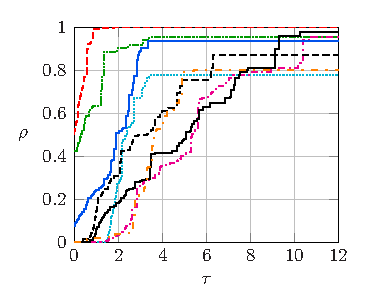
\includegraphics{lexample_fig1}
%     \caption{Example figure using external image files.}
%     \label{fig:testfig}
%   \end{figure}
%   \Cref{tab:foo} shows additional
%   supporting evidence.
% }
% \textcolor{gray}{
%   \begin{table}[htbp]
%     \footnotesize
%     \caption{Example table.}\label{tab:foo}
%     \begin{center}
%       \begin{tabular}{|c|c|c|} \hline
%         Species & \bf Mean & \bf Std.~Dev. \\ \hline
%         1       & 3.4      & 1.2           \\
%         2       & 5.4      & 0.6           \\
%         3       & 7.4      & 2.4           \\
%         4       & 9.4      & 1.8           \\ \hline
%       \end{tabular}
%     \end{center}
%   \end{table}
% }

% \section{Discussion of \texorpdfstring{{\boldmath$Z=X \cup Y$}}{Z = X union Y}}


% \section{Remarks}
% \label{sec:remarks}

% some remarks.

% In \cref{thm:regularity}
% If \(f\in L^\infty(\Omega)\)  then \(u \in C_{\alpha/2}(\Omega)\), which is Proposition 1.1 in \cite{ROSOTON2014275}.

% When \(\|f\|_{\beta}^{(\gamma)} < \infty\), where \(\beta > 2-\alpha\) and \(\gamma \in [-\alpha, -\alpha/2]\), we observed convergent order \(\min\{r(\alpha+\gamma), 2\}\) in numerical experiments. 
% And we can prove that kind theorems with the techneque we used in this paper. 
















\appendix

\section{Approximate of difference quotients}

\begin{lemma} \label{lmm:Dh2simd2}
  If \(g(x)\in C^2(\Omega)\),
  there exists \(\xi\in (x_{i-1}, x_{i+1})\) such that
  \begin{equation} \label{eq:Dh2simd2}
    \begin{aligned}
      D_h^2 g(x_i) & = g''(\xi), \quad \xi \in (x_{i-1}, x_{i+1})
    \end{aligned}
  \end{equation}
  % \begin{equation} \label{eq:Dh2Cauchy2}
  %   \begin{aligned}
  %      & \frac{2}{h_i + h_{i+1}} \left( \frac{1}{h_{i+1}} g(x_{i+1}) - (\frac{1}{h_{i}}+\frac{1}{h_{i+1}})g(x_{i}) + \frac{1}{h_{i}} g(x_{i-1}) \right)                          \\
  %     % &= \frac{h_i}{h_i + h_{i+1}} g''(\xi_1) + \frac{h_{i+1}}{h_i + h_{i+1}} g''(\xi_2)  \\
  %      & \quad = \frac{2}{h_i + h_{i+1}} \left( \frac{1}{h_{i}}\int_{x_{i-1}}^{x_i} g''(y) (y-x_{i-1}) dy + \frac{1}{h_{i+1}} \int_{x_i}^{x_{i+1}} g''(y) (x_{i+1}-y) dy \right)
  %   \end{aligned}
  % \end{equation}
  And if \(g(x) \in C^4(\Omega)\), then
  \begin{equation} \label{eq:Dh2simd4}
    \begin{aligned}
      D_h^2 g(x_i) &= g''(x_{i}) + \frac{h_{i+1}-h_{i}}{3} g'''(x_{i}) \\
      &\quad  +  \frac{2}{h_i + h_{i+1}}\left( \frac{1}{h_{i}}\int_{x_{i-1}}^{x_i} g''''(y) \frac{(y-x_{i-1})^3}{3!} dy + \frac{1}{h_{i+1}} \int_{x_i}^{x_{i+1}} g''''(y) \frac{(x_{i+1}-y)^3}{3!} dy \right)  \\
    \end{aligned}
  \end{equation}
\end{lemma}
\begin{proof}
  \begin{gather*}
    g(x_{i-1}) = g(x_{i}) - (x_{i}-x_{i-1}) g'(x_{i}) + \frac{(x_{i}-x_{i-1})^2}{2} g''(\xi_1), \quad \xi_1 \in (x_{i-1}, x_{i})        \\
    g(x_{i+1}) = g(x_{i}) + (x_{i+1}-x_{i}) g'(x_{i}) + \frac{(x_{i+1}-x_{i})^2}{2} g''(\xi_2), \quad \xi_2 \in (x_{i}, x_{i+1})
  \end{gather*}
  Subsitute them in the left side of \eqref{eq:Dh2simd2}, we have
  \begin{equation*}
    \begin{aligned}
      D_h^2 g(x_i) & = \frac{2}{h_i + h_{i+1}} \left( \frac{1}{h_{i+1}} (g(x_{i+1})-g(x_i)  + \frac{1}{h_{i}} (g(x_{i-1})-g(x_i)) \right) \\
      &= \frac{h_i}{h_i + h_{i+1}} g''(\xi_1) + \frac{h_{i+1}}{h_i + h_{i+1}} g''(\xi_2)
    \end{aligned}
  \end{equation*}
  Now, using \textcolor{red}{intermediate value theorem}, there exists \(\xi \in [\xi_1, \xi_2]\) such that
  \begin{equation*}
    \frac{h_i}{h_i + h_{i+1}} g''(\xi_1) + \frac{h_{i+1}}{h_i + h_{i+1}} g''(\xi_2) = g''(\xi)
  \end{equation*}
  % For the second equation, similarly
  % \begin{gather*}
  %   g(x_{i-1}) = g(x_{i}) - (x_{i}-x_{i-1}) g'(x_{i}) + \int_{x_{i-1}}^{x_i} g''(y) (y-x_{i-1}) dy \\
  %   g(x_{i+1}) = g(x_{i}) + (x_{i+1}-x_{i}) g'(x_{i}) + \int_{x_i}^{x_{i+1}} g''(y) (x_{i+1}-y) dy
  % \end{gather*}
  And the last equation can be obtained by
  \begin{gather*}
    g(x_{i-1}) = g(x_{i}) - h_{i} g'(x_{i}) + \frac{h_{i}^2}{2} g''(x_{i}) - \frac{h_{i}^3}{3!} g'''(x_{i}) +  \int_{x_{i-1}}^{x_{i}} g''''(y) \frac{(y-x_{i-1})^3}{3!} dy        \\
    g(x_{i+1}) = g(x_{i}) + h_{i+1} g'(x_{i}) + \frac{h_{i+1}^2}{2} g''(x_{i}) + \frac{h_{i+1}^3}{3!} g'''(x_{i}) + \int_{x_{i}}^{x_{i+1}} g''''(y) \frac{(x_{i+1}-y)^3}{3!} dy
  \end{gather*}
  Expecially,
  \begin{equation} \label{eq:Dh2Cauchy4}
    \begin{aligned}
      \int_{x_{i-1}}^{x_{i}} g''''(y) \frac{(y-x_{i-1})^3}{3!} dy & = \frac{h_i^4}{4!}g''''(\eta_1) \\
      \int_{x_{i}}^{x_{i+1}} g''''(y) \frac{(x_{i+1}-y)^3}{3!} dy & = \frac{h_{i+1}^4}{4!}g''''(\eta_2)
    \end{aligned}
  \end{equation}
  where \(\eta_1 \in (x_{i-1}, x_{i}), \eta_2 \in (x_{i}, x_{i+1})\).
\end{proof}


\begin{lemma} \label{lmm:Dyj}
  Denote \(y_j^\theta = (1-\theta) x_{j-1} + \theta x_j, \theta\in (0,1)\),
  % then for \(2\le j \le 2N-1\)
  \begin{equation}
    \begin{aligned}
      u(y_j^\theta) - \Pi_hu(y_j^\theta) & = -\frac{\theta (1-\theta)}{2} h_j^2 u''(\xi), \quad \xi \in (x_{j-1}, x_j)
    \end{aligned}
  \end{equation}
  \begin{equation}
    \begin{aligned}
      u(y_j^\theta) - \Pi_hu(y_j^\theta) = & -\frac{\theta (1-\theta)}{2} h_j^2 u''(y_j^\theta)
      + \frac{\theta (1-\theta)}{3!} h_j^3 (\theta^2 u'''(\eta_1) - (1-\theta)^2 u'''(\eta_2))
    \end{aligned}
  \end{equation}
  where \(\eta_1 \in (x_{j-1}, y_j^\theta), \eta_2 \in (y_j^\theta, x_j)\).
\end{lemma}
\begin{proof}
  By Taylor expansion, we have
  \begin{gather*}
    u(x_{j-1}) = u(y_j^\theta) - \theta h_{j} u'(y_j^\theta) + \frac{\theta^2 h_{j}^2}{2!} u''(\xi_1), \quad \xi_1 \in (x_{j-1}, y_j^\theta) \\
    u(x_{j}) = u(y_j^\theta) + (1-\theta) h_{j} u'(y_j^\theta) + \frac{(1-\theta)^2 h_{j}^2}{2!} u''(\xi_2) , \quad \xi_2 \in (y_j^\theta, x_j)
  \end{gather*}
  Thus
  \begin{equation*}
    \begin{aligned}
      u(y_j^\theta) - \Pi_hu(y_j^\theta) 
      & = u(y_j^\theta) - (1-\theta) u(x_{j-1}) - \theta u(x_{j})      \\
      & = -\frac{\theta (1-\theta)}{2} h_j^2 ( \theta u''(\xi_1) + (1-\theta) u''(\xi_2) ) \\
      & = -\frac{\theta (1-\theta)}{2} h_j^2 u''(\xi), \quad \xi \in [\xi_1, \xi_2]
    \end{aligned}
  \end{equation*}
  The second equation is similar,
  \begin{gather*}
    u(x_{j-1}) = u(y_j^\theta) - \theta h_{j} u'(y_j^\theta) + \frac{ \theta^2h_{j}^2}{2!} u''(y_j^\theta) - \frac{\theta^3 h_{j}^3}{3!} u'''(\eta_1)  \\
    u(x_{j}) = u(y_j^\theta) + (1-\theta) h_{j} u'(y_j^\theta) + \frac{(1-\theta)^2 h_{j}^2}{2!} u''(y_j^\theta) + \frac{(1-\theta)^3 h_{j}^3}{3!} u'''(\eta_2)
  \end{gather*}
  where \(\eta_1 \in (x_{j-1}, y_j^\theta), \eta_2 \in (y_j^\theta, x_j)\).
  Thus
  \begin{equation*}
    \begin{aligned}
      u(y_j^\theta) - \Pi_hu(y_j^\theta) 
      & = u(y_j^\theta) - (1-\theta) u(x_{j-1}) -\theta u(x_{j})   \\
      & = -\frac{\theta (1-\theta)}{2} h_j^2 u''(y_j^\theta) + \frac{\theta (1-\theta)}{3!} h_j^3 ( \theta^2 u'''(\eta_1) - (1-\theta)^2 u'''(\eta_2))
    \end{aligned}
  \end{equation*}
\end{proof}

\begin{lemma} \label{lmm:Dyjleh2ya/2m2/r}
  By \cref{lmm:Dyj}, \cref{cor:regularity-u} and \cref{lmm:hilexi} ,
  There is a constant \(C=C(T, \alpha, r, \|u\|_{\beta+\alpha}^{(-\alpha/2)})\) for \(2\le j \le 2N-1\),
  \begin{equation}
    |u(y)-\Pi_hu(y)| \le h_j^2 \max_{\xi\in [x_{j-1}, x_j]}|u''(\xi)| \le C h^2 \delta(y)^{\alpha/2-2/r}, \quad \text{for } y\in (x_{j-1}, x_{j})
  \end{equation}
\end{lemma}

\begin{lemma} \label{lmm:Dyj1}
  For \(x\in [x_{j-1}, x_j]\)
  \begin{equation}
    \begin{aligned}
      |u(x) - \Pi_hu(x)| & = \left| \frac{x_{j}-x}{h_j} \int_{x_{j-1}}^x u'(y) dy - \frac{x-x_{j-1}}{h_j} \int_{x}^{x_{j}} u'(y) dy \right| \\
                      & \le \int_{x_{j-1}}^{x_{j}} |u'(y)| dy
    \end{aligned}
  \end{equation}
  If \(x\in [0, x_1]\), with \cref{cor:regularity-u}, we have
  \begin{equation}
    |u(x) - \Pi_hu(x)| \le \int_{0}^{x_1} |u'(y)| dy \le \int_{0}^{x_1} C y^{\alpha/2-1} dy  \le C\frac{2}{\alpha} x_1^{\alpha/2} = C\frac{2}{\alpha} h_1^{\alpha/2}
  \end{equation}
  Similarly, if \(x\in [x_{2N-1}, 1]\), we have
  \begin{equation}
    |u(x) - \Pi_hu(x)| \le C\frac{2}{\alpha} (2T-x_{2N-1})^{\alpha/2} = C\frac{2}{\alpha} h_{2N}^{\alpha/2}
  \end{equation}
\end{lemma}


\begin{lemma} \label{ineq:a-b-theta}
  \begin{equation}
    b^{1-\theta}|a^{\theta}-b^{\theta}| \le |a-b| \; (\text{  also  }a^{1-\theta}|a^{\theta}-b^{\theta}| \le |a-b|), \quad a,b\ge 0,\; \theta \in [0,1]
  \end{equation}
\end{lemma}




\section{Proofs of some technical details}

Review that \(h=\frac{1}{N}\) and the defination of \(\simeq\) in \cref{sec:numformat}




\textcolor{blue}{
  \begin{lemma} \label{lmm:hi1-hi}
    There is a constant \(C\) such that for \(i=1,2,\cdots,2N-1\)
    \begin{equation}
      |h_{i+1} - h_{i}| \le C h^2 \delta(x_i)^{1-2/r} 
    \end{equation}
  \end{lemma}
  \begin{proof}
    By \cref{def:hj},
    \begin{equation}
      \begin{aligned}
        h_{i+1} - h_{i} =
        \begin{cases}
          T \left( \left(\frac{i+1}{N}\right)^r - 2\left(\frac{i}{N}\right)^r + \left(\frac{i-1}{N}\right)^r  \right) ,           & 1\le i\le N-1    \\
          0,    & i=N    \\
          -T \left( \left(\frac{2N-i-1}{N}\right)^r - 2\left(\frac{2N-i}{N}\right)^r + \left(\frac{2N-i+1}{N}\right)^r  \right) , & N+1\le i\le 2N-1 \\
        \end{cases}
      \end{aligned}
    \end{equation}
    Since
    \begin{equation}
      (i+1)^r - 2i^r + (i-1)^r \simeq r(r-1)i^{r-2}, \quad \text{for  } i\ge 1
    \end{equation}
    We get the result.
  \end{proof}
}




\begin{lemma} \label{lmm:trucerr2d2f}
  there is a constant \(C=C(T, \alpha, r, \|f\|_{\beta}^{\alpha/2})\) such that
    \begin{equation}
      \begin{aligned}
        & \frac{2}{h_i + h_{i+1}} \left| \frac{1}{h_i} \int_{x_{i-1}}^{x_{i}} f''(y) \frac{(y-x_{i-1})^3}{3!} dy + \frac{1}{h_{i+1}} \int_{x_{i}}^{x_{i+1}} f''(y) \frac{(y-x_{i+1})^3}{3!} dy \right| \\
         & \quad \le C h^2 \delta(x_i)^{-\alpha/2-2/r} 
      \end{aligned}
    \end{equation}
\end{lemma}
\begin{proof} \label{prf:trucerr2d2f}
  By \cref{thm:regularity-f}, we have for \(1 \le i \le N\)
  \begin{equation}
    \begin{aligned}
      \left|\int_{x_{i-1}}^{x_{i}} f''(y)\frac{(y-x_{i-1})^3}{3!} dy \right|  \le \frac{\|f\|_{\beta}^{(\alpha/2)}}{3!} \int_{x_{i-1}}^{x_{i}} y^{-\alpha/2-2} (y-x_{i-1})^3 dy
    \end{aligned}
  \end{equation}
  For \(i=1\),
  \begin{equation*}
    \int_{x_{i-1}}^{x_{i}} y^{-\alpha/2-2} (y-x_{i-1})^3 dy
    = \int_{0}^{x_{1}} y^{1-\alpha/2} dy
    = \frac{1}{2-\alpha/2} x_1^{2-\alpha/2} = \frac{1}{2-\alpha/2} x_1^{-\alpha/2-2} h_1^4
  \end{equation*}
  And for \(2\le i \le N\), since \(x_i\simeq x_{i-1}\le y\le x_i\), we have
  \begin{equation*}
    \begin{aligned}
      \int_{x_{i-1}}^{x_{i}} y^{-\alpha/2-2} (y-x_{i-1})^3 dy
      \simeq \int_{x_{i-1}}^{x_{i}} x_i^{-\alpha/2-2} (y-x_{i-1})^3 dy
      = \frac{1}{4!} x_i^{-\alpha/2-2} h_i^4
    \end{aligned}
  \end{equation*}
  So for  \(1\le i\le N\), we have 
  \begin{equation}
    \left|\int_{x_{i-1}}^{x_{i}} f''(y)\frac{(y-x_{i-1})^3}{3!} dy \right| \le C x_i^{-\alpha/2-2} h_i^4
  \end{equation}
  and similarly,
  \begin{equation}
    \left|\int_{x_{i}}^{x_{i+1}} f''(y)\frac{(x_{i+1}-y)^3}{3!} dy \right| \le C x_i^{-\alpha/2-2} h_{i+1}^4
  \end{equation}
  Thus for \(1\le i\le N\), with \cref{lmm:hilexi} we have
  \begin{equation}
    \begin{aligned}
      & \frac{2}{h_i + h_{i+1}} \left| \frac{1}{h_i} \int_{x_{i-1}}^{x_{i}} f''(y) \frac{(y-x_{i-1})^3}{3!} dy + \frac{1}{h_{i+1}} \int_{x_{i}}^{x_{i+1}} f''(y) \frac{(y-x_{i+1})^3}{3!} dy \right| \\
       & \quad \le C x_i^{-\alpha/2-2} \frac{2}{h_i + h_{i+1}} (h_i^3 + h_{i+1}^3)
       \simeq x_i^{-\alpha/2-2} h_i^2 \simeq x_i^{-\alpha/2-2} h^2 x_i^{2-2/r} \\
       &\quad = C h^2 x_i^{-\alpha/2-2/r}
    \end{aligned}
  \end{equation}
  It's symmetric for \(N < i \le 2N-1\).
\end{proof}

\begin{lemma} \label{lmm:Dh2Kyxi}
  There is a constant \(C=C(\alpha, r)\) such that for all \(1 \le i \le 2N-1\), \(1\le j \le 2N\) s.t. \(\min\{|j-i|, |j-1-i|\} \ge 2\) and \(y\in [x_{j-1}, x_{j}]\), we have
  \begin{equation}
    D_h K_y (x_i) \simeq |y - x_i|^{-\alpha} ,\quad
    D_h^2 K_y (x_i) \simeq |y-x_i|^{-1-\alpha}
  \end{equation}
\end{lemma}
\begin{proof}
  Sinec \(y-x_{i-1}, y-x_{i}, y-x_{i+1}\) have the same sign, by mean value theorem and \cref{lmm:Dh2simd2},
  \begin{equation*}
    \begin{aligned}
      D_h K_y (x_i) &= \frac{|y-\xi|^{-\alpha}}{\Gamma(1-\alpha)}, \quad \xi\in (x_{i}, x_{i+1})  \\
      D_h^2 K_y (x_i) & = \frac{|y-\xi|^{-1-\alpha}}{\Gamma(-\alpha)}, \quad \xi\in (x_{i-1}, x_{i+1})
    \end{aligned}
  \end{equation*}
  however, \(|y - \xi| \simeq |y - x_i|\) , we get the result.
\end{proof}


\begin{lemma} \label{lmm:sumSij13}
  There exists a constant \(C=C(T, \alpha, r, \|u\|_{\beta+\alpha}^{(-\alpha/2)})\) such that
  \begin{gather}
    \sum_{j=1}^{3} V_{1j} \le C h^2 x_1^{-\alpha/2-2/r}\\
    \sum_{j=1}^{4} V_{2j} \le C h^2 x_2^{-\alpha/2-2/r}
  \end{gather}
\end{lemma}
\begin{proof}
  For \(0\le i \le 3, 1\le j \le 4\), by \cref{lmm:Dyj1}, \cref{lmm:Dyjleh2ya/2m2/r} and \cref{def:Tij}
  \begin{equation}
    T_{ij} \le C x_1^{2-\alpha/2} \simeq h_1^2 \; h^2 x_1^{-\alpha/2-2/r} \simeq h_1^2 \; h^2 x_2^{-\alpha/2-2/r}
  \end{equation}
  Therefore, by \cref{def:Vij}, we get the result.
\end{proof}




\section*{Acknowledgments}
\textcolor{gray}{
  We would like to acknowledge the assistance of volunteers in putting
  together this example manuscript and supplement.
}
\bibliographystyle{siamplain}
\bibliography{references}
\end{document}
